%!TEX root = article.tex

\section{Appendix}
\label{s:Appendix}

%Additional material such as extra figures.

\subsection{Additional Material for the Green's Function Method}
%Put all the extra plots etc. from Green's Function Code here.

\subsubsection{General Structure of the Used Code}
\label{GreensCode}
%Explain everything about the code

In this section, an insight to the code provided by Secomb et al. \cite{Secomb2004} will be given. Especially a description about what data this code uses and what data it computes will follow.. 
The main goal is to understand what the results are and where they really come from. For this, a general explanation of the structure and organization of the code and the methods behind the computations will given.

\subsubsection*{Inputs}
\label{Inputs}
%What data this code actually needs and what this data is
%What are the inputs for this code ? Where do they come from ?

In general, the Green's function method code takes .dat-files as inputs, which basically contain the network files and the parameters for the diffusion and oxygen transport inside the vessels.
\\
\\The input data in form of .dat-files consists of four files:\\
\\- The SoluteParams.dat-file: This file contains all the information about the solutes we are looking at. In our case, this is simply oxygen. The specific informations are things like the tissue solubility, the Michaelis constant of consumption, etc.\\
\\- The Network.dat-file: This file contains all the information about the network we are looking at. This information is basically in form of an array. This array defines for each segment the type of vessel, the start point, the end point, the diameter (in microns), the relativ flow and the hematocrit level of the blood inside the given vessel.\\
\\- The IntravascRes.dat-file: This file contains all the information about the diameter on which the sources are computed around the vessel centerline. The second important information given here is the intravascular resistance to radial oxygen transport $K$ for each diameter and vessel.\\
\\- The ContourParams.dat-file: This file contains all the information necessary to create the contour-plots. This means that we create a plot, where the oxygen concentration inside a three dimensional domain can be visualized on a two dimensional projection. In this file, the projection plane can be specified, and the focus geometry inside the three dimensional space can be selected.
\\
\\The part of the code where the read-in of the network data and the specific transport parameters through the input files is being done is the input.cpp code.
\\
\\The analyzenet.cpp-part of the code analyzes the input-files and gives each vessel and node a number. Through this, the oxygen concentration can be computed for each node of the three dimensional space. The output after this step can be seen in Figure \ref{fig:NetNodesSegs_Glom}, but it is important to note that usually in the next step, the oxygen gradients are computed, and the segmentation numbers are replaced by the specific oxygen levels for each node and vessel.

\subsubsection*{Outputs}
\label{Outputs}
%What this code actually produces
%What are the outputs for this code ? How are they produced ? Where do they come from ?

The Green's function method code gives .dat-files and images (contour.ps-files) as outputs, which basically contain the results that have been discussed previously in the Results \ref{Results} chapter.
\\
\\The contour.ps-files are produced by the contour.cpp-part of the code, which basically generates and writes the data for the contour-plots. This data is a plot of the vessel from bottom to top according to the z-coordinate. In other words, this is a two dimensional projection of the computed oxygen fields in a three dimensional space. One could see this plot as a 2D picture of a 3D network, giving some information about the general oxygen fields everywhere in the segment. There is an option of computing the transport of different solutes in the network, in which case a new page is generated for each solute, and the computed solute concentration for each area is shown in colors. In our case, the only used solute is oxygen and thus only one contour-plot is shown for each network.
\\
%contr-lines
\\The lines on the contour plots are generated by the contr-lines.cpp-part of the code, whereas the contr-shade.cpp-part generates the colors and the color bar on the side of the generated contour-plots.
\\
\\The code responsible for the creation of the NetNodesSegs.ps and the NedNodesOxygen.ps-files is picturenetwork.cpp. Here, the network and the computed oxygen fields of the network are projected on a z = 0 plane. For this, the parameters from the CountourParams.dat file are used. Finally, a postscript file called NetNodesSegs is produced, in which nodes are labeled with nodvar and segments with segvar. A second file called NetNodesOxygen is produced, in which the computed oxygen level for each node is pictured.
\\
\newpage
The general outputs of the code can be classified into two categories:\\
\\- The first category is in the form of PostScript-files that can be visualized. These outputs are basically pictures showing the computed oxygen concentrations. The three files are the ones that were previously mentioned: the Contour.ps-file, the NedNodesSegs.ps-file and finally the NedNodesOxygen.ps-file.\\
\\- The second category is in the form text-files, containing the computed data in arrays. These values are the computed oxygen partial pressures for each node in the tissue, and represent the oxygen field output for a three-dimensional segment.
\\

\subsubsection*{Organization of the Code}
%Briefly talk about each part of the code and explain how it all works together
%Might keep this part more general and mention each of the parts of the code like a puzzle in the Appendix

The code provided by Secomb et al. \cite{Secomb2004} consists of a few .cpp-files, so that tasks like input read-ins, calculations and output-file generations are separated. Each file has a specific role, which will be explained in detail in this section. As one can think, the most important part of this code is the implementation of the Green's function method and its application to the given data.
\\
\begin{itemize}
%Solver bicgstab
 \item The solver:
\\The bicgstab.cpp-part of the code is the implementation of a solver based on the Parameter-free iterative linear solver by R. Weiss \cite{weiss1996parameter}.
%blood
\\ \item $O_2$ partial pressure computation:
\\The blood.cpp-part of the code is quite interesting, as it basically does an important part of the calculation to obtain the oxygen concentration field in the vessels and the tissue. In this part of the code, the partial pressure of oxygen is computed depending on the oxygen concentration in the red blood cells. The oxygen concentration in the red blood cells is taken as an input and the partial pressure of oxygen is given as an output for each node. This step is then repeated iteratively as the results for the computed oxygen field is converging.
%convect
\\ \item Computation of the convective flux:
\\ The convect.cpp-part of the code does the convective transport part of the calculation. It examines the flow direction, to compute the oxygen concentration in each vessel segment in the right order.
%eval
\newpage
 \item Evaluation of solute fields:
\\The eval.cpp-part of the code does the evaluation of the solute field depending on the source strengths provided. As mentioned previously, the source strength field is computed after a first random guess, and the solute concentration field calculations are being done iteratively starting from this guess.
%numerical methods (gaussj and ludcmp)
\\ \item Numerical methods:
\\There are some numerical methods and mathematical calculations behind the simulation, as for example the \emph{Gauss-Jordan elimination} or the \emph{Lower-Upper decomposition}, which have not been studied in detail for the purposes of this thesis, but are implemented in the gaussj.cpp-part and the ludcmp.cpp-part of the code.
%greens
\\ \item Green's method:
\\The main implementation of the Green's function method is in the greens.cpp-part of the code. Here the Green's function approach for multiple reacting species is applied. The equations described in the Methods \ref{Greens} section are implemented to compute the oxygen partial pressure $PO_2$.
%histogram
\\ \item Histogram computation:
\\In this part, histograms of the solute levels are evaluated, and a histogram.dat-file is generated as an output. This file has the form of a text-document, and contains a array with the data.
%initgreens
\\ \item Initial guessing of the source field:
\\As previously mentioned, a guess for the initial tissue source strengths is being done. Later, the source strength is computed iteratively and the computed sink field depends on this calculation. This is due to the Michaelis-Menten relation we are using to calculate the oxygen consumption. For this reason, the initgreens.cpp-part of the code is only used at the beginning of each simulation.
%main
%\\The code main.cpp calls the greens.cpp-code.
%\\
%nrutil (.cpp and .hh)
%\\The code nrutil.cpp/nrutil.hh is declaring variables and is allocating them.
%\\
%outboun (method?)
%\\ \item Linear interpolation:
%\\Outboun.cpp: method = 1: finds the smallest convex region inside the cuboid which excludes tissue node points that have a distance to the nearest vessel greater than a value specified by the user (lb).  Any point outside a region between two planes containing the required points is excluded.  This is repeated for multiple plane orientations, determined by am.
%\\
%\\method = 2: finds all tissue points within a distance lb of the vessels, but does not make a convex region.  Fills in 'holes' in interior, whether 2D or 3D.
%\\
%\\Output:	nnt, total tissue node points inside the region. nbou > 1 if inside region, value gives tissue point index
%\\
%putrank
\\ \item Node generation:
\\The direction of the flow is an essential information which we have to take care of, in order to get physically accurate results. For this, the nodes have be generated in the right order. The rank of the node is exactly the information pictured on the output NetNodesSegs.ps. For this, the putrank.cpp-code generates nodes in order of flow direction, depending on the physical direction of the flow.
%readsources (new --> is not used yet)
%\\ \item Source reading and array setting:
%\\readsources.cpp: read source strengths from file (from TissueSources.out and VesselSources.out)
%\\
%setuparrays 0, 1, 2
\\ \item Array generation:
\\Arrays with fixed dimensions, as for example vessel segments, have to be generated. This is done by the setuparray.cpp-part of the code, where the dimensions of segments is set.
%\\setuparrays0.cpp: set up arrays with fixed dimensions (for Green's)
%\\
%\\setuparrays1.cpp: set up arrays with dimensions of nnod and nseg (for Green's)
%\\
%\\setuparrays2.cpp: set up arrays with dimensions of nnv and nnt (for Green's)
%testconvect
\\ \item Testing the convection direction:
\\The correctness of the direction in the convective flow is tested by comparing the matrix values with values obtained by numerical differentiation. This is done in the testconvect.cpp-part of the code.
%tissrate
\\ \item Calculation of the uptake rate:
\\In the tissrate.cpp-part of the code, the uptake rate of the computed solutes (in our case it is only oxygen) in the tissue is computed as a function of solute levels. This means in our case, that the tissue uptake (the diffusion and the myoglobin enhanced transport) of oxygen is calculated depending on the concentration surrounding the given tissue.
\\
%Everyone of these code-parts is using the nrutil.hh code, why ?
\end{itemize}

\subsubsection{Some More Green's Results}

\begin{figure}[h]
\centering
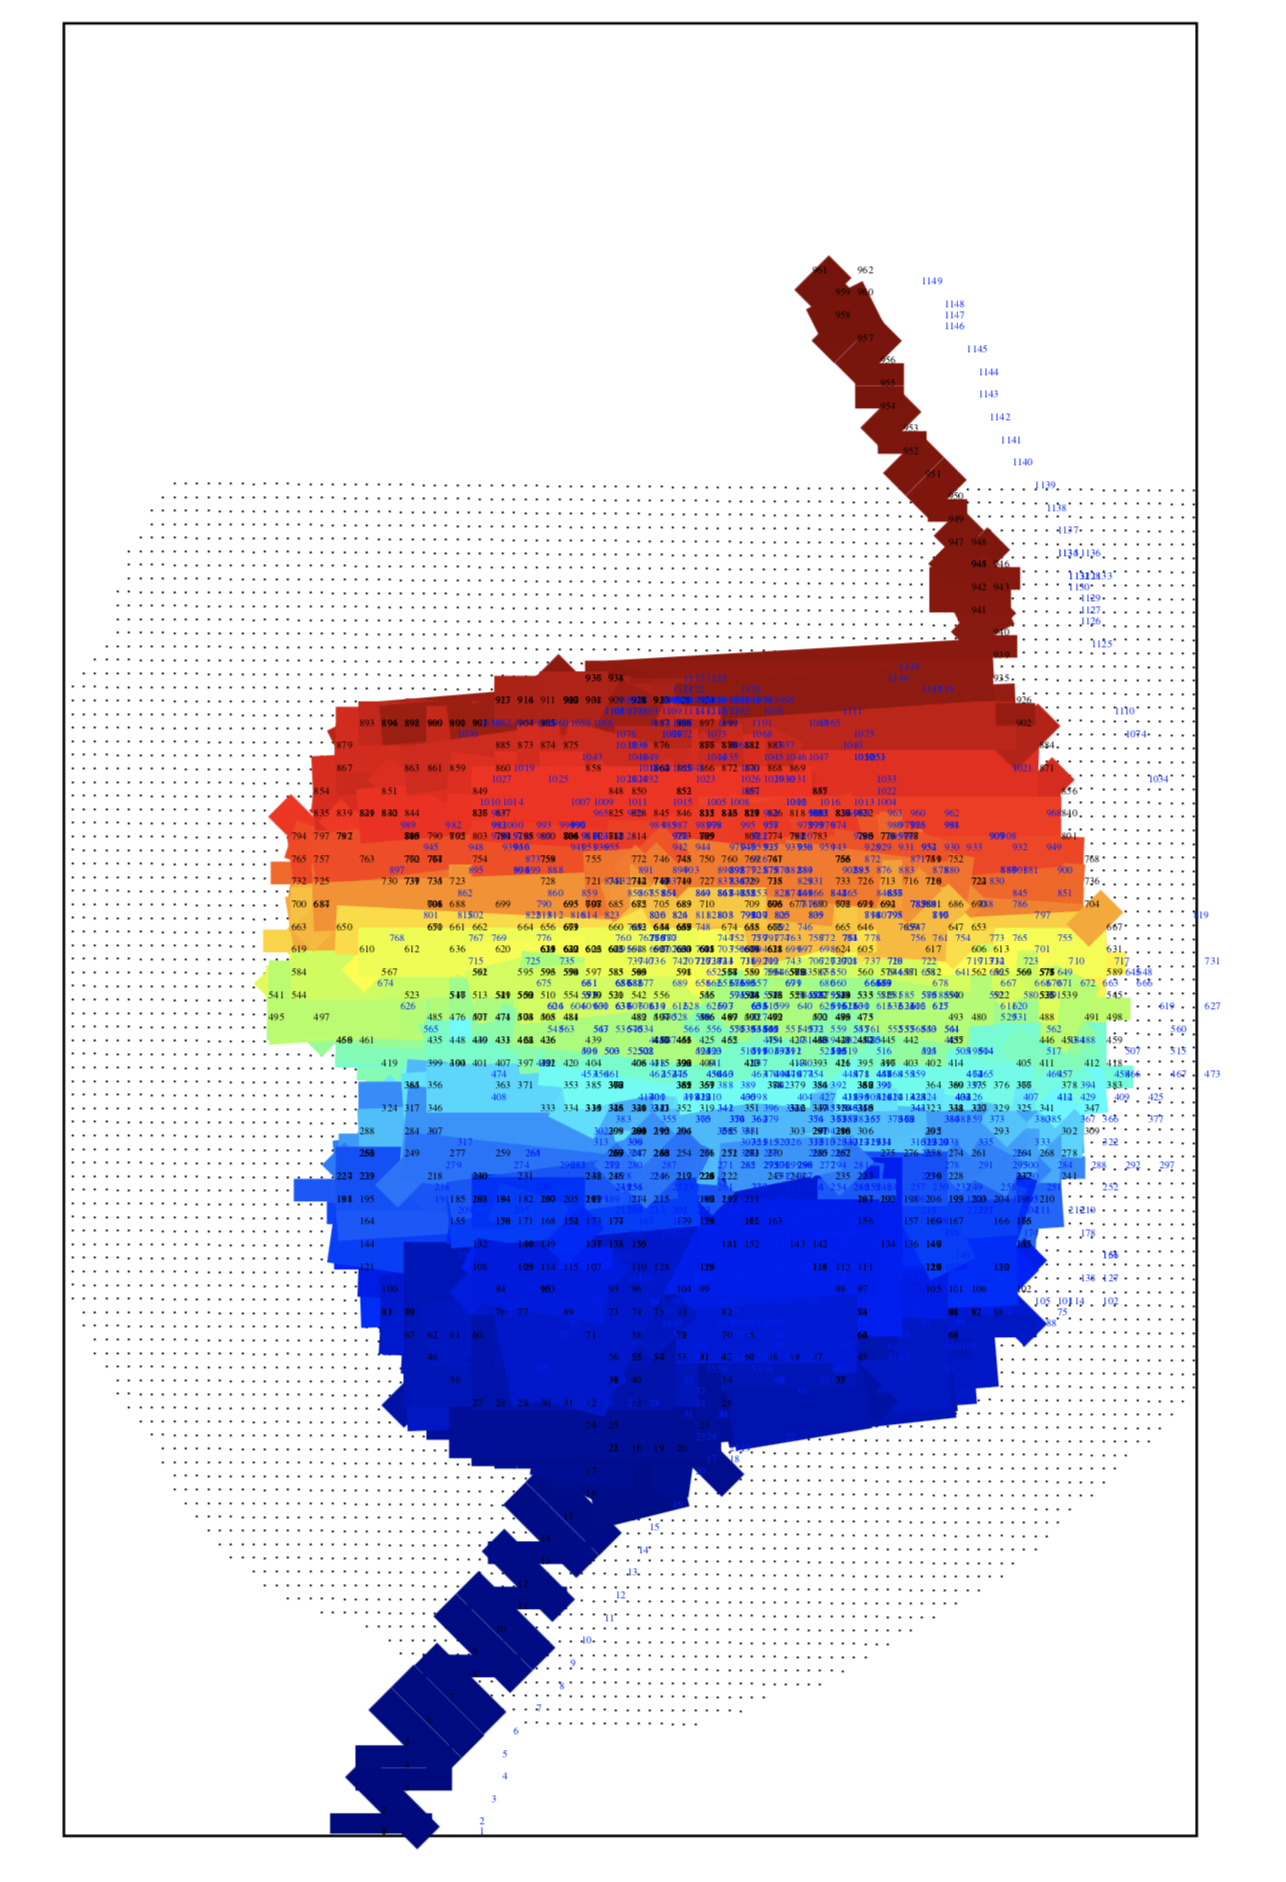
\includegraphics[width=100mm]{NetNodesSegs_Glom}
\caption{\footnotesize Green's Net Nodes Output for a Glomerulus Network}
\label{fig:NetNodesSegs_Glom}
\end{figure}
The figure \ref{fig:NetNodesSegs_Glom} shows the previously mentioned NetNodesSegs.ps output computed for a glomerulus network. One can see that a number (or more precisely a rank) is assigned to each vessel segment and to each node. This step is the first step that has to be done before any computations concerning oxygen fields in the vessels and the tissue can be done.

\subsection{Additional Material for DuMuX}
%Put all the extra images from ParaView here.

%\newpage
%\subsubsection{Some Glomerulus Network Simulation Results}
%Just to have some more figures

%\begin{figure}[h]
%\centering
%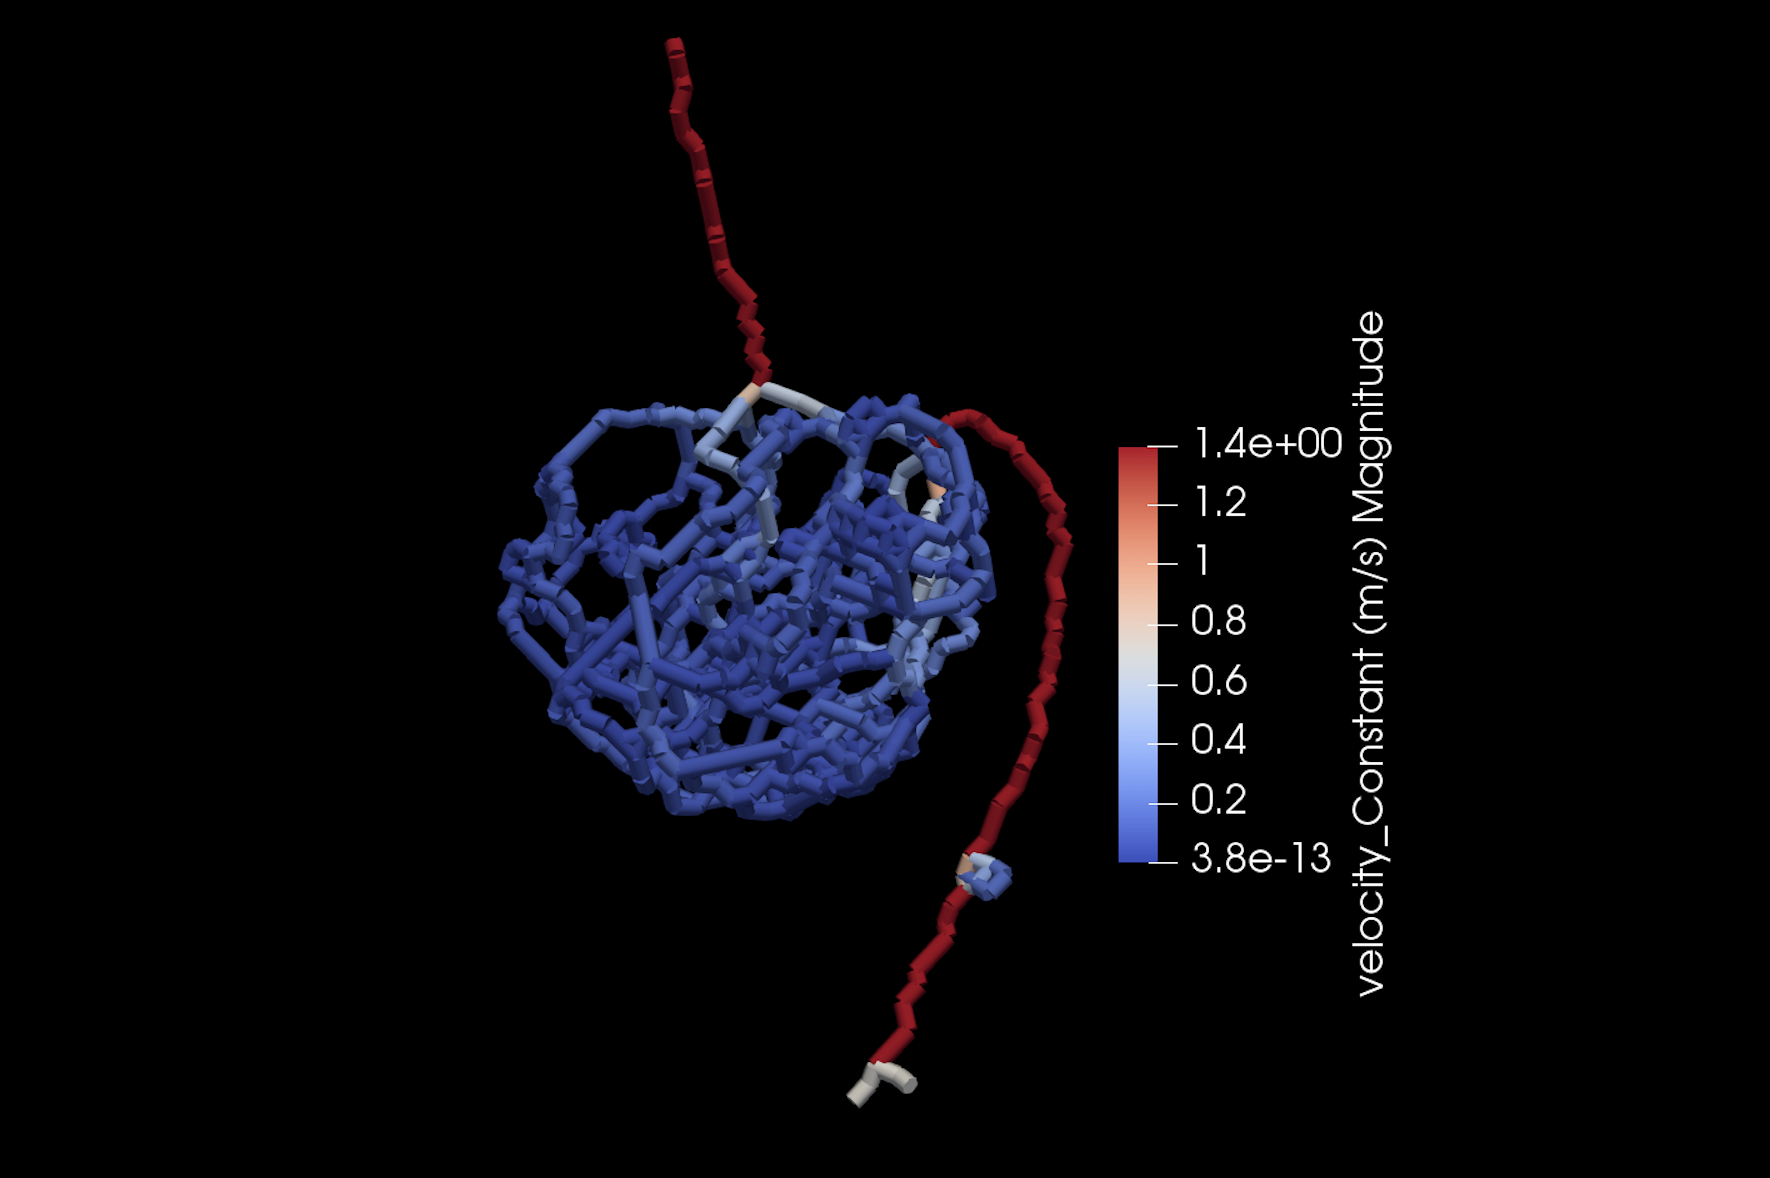
\includegraphics[width=162mm]{glom_velocity}
%\caption{Velocity Field in a Glomerulus}
%\label{fig:glom_velocity}
%\end{figure}
%The figure \ref{fig:glom_velocity} is the result of a DuMuX 1p-1p blood flow simulation computed on a glomerulus network. The velocity field of the flow is visualized.\\

%\begin{figure}[h]
%\centering
%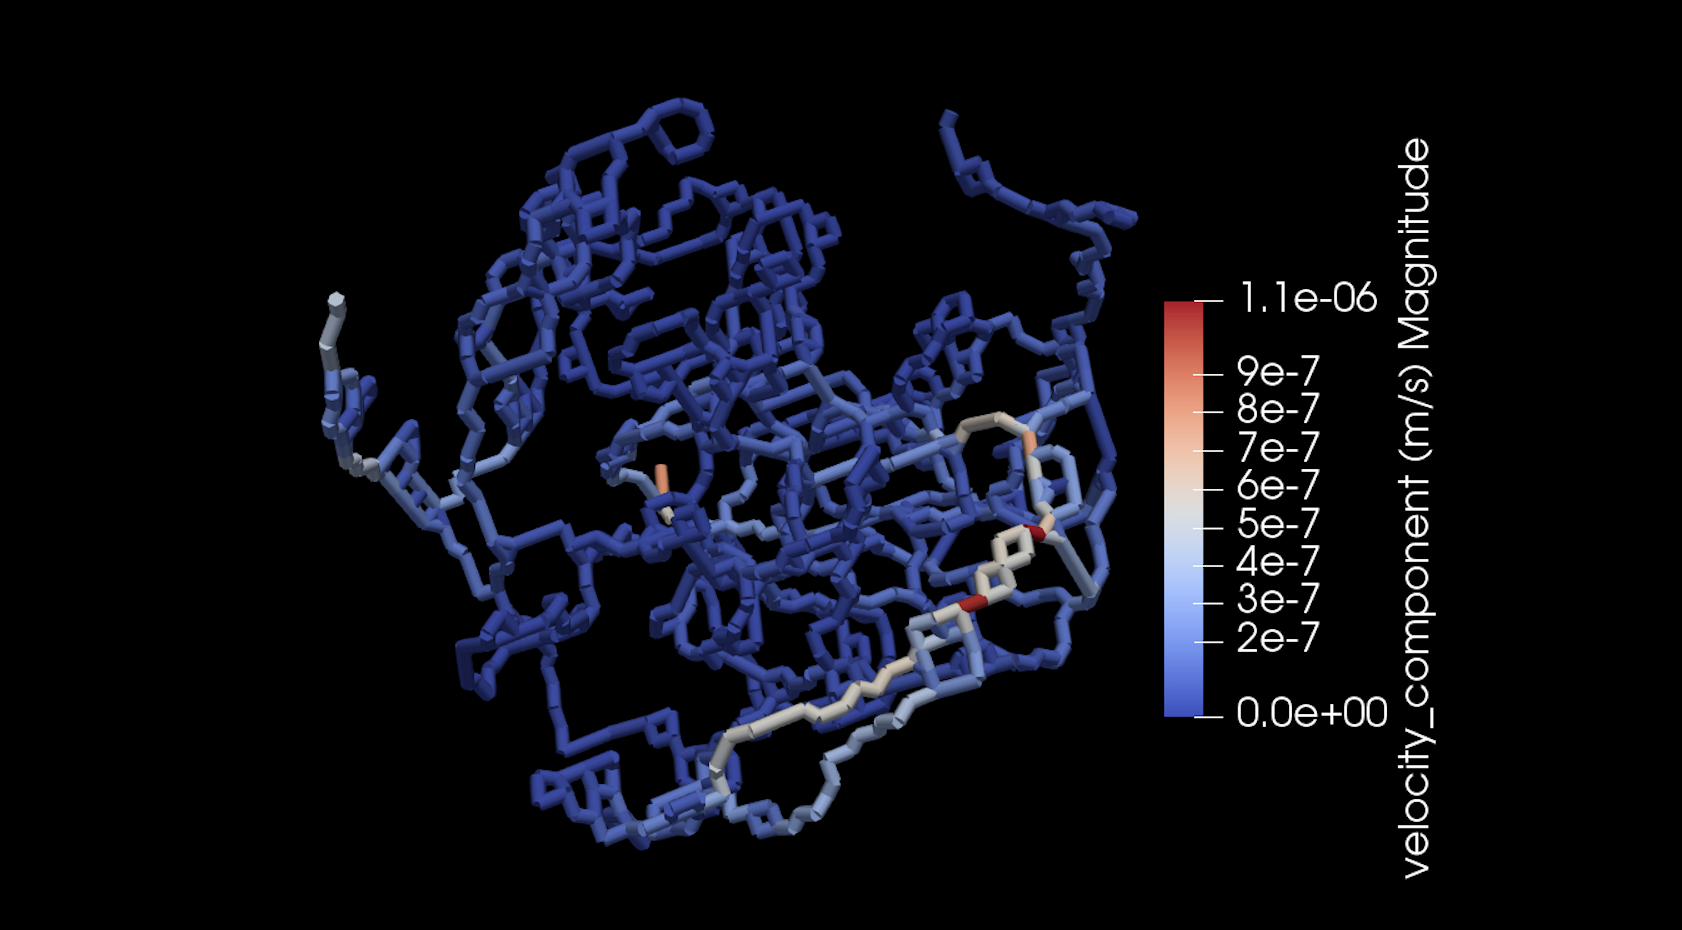
\includegraphics[width=162mm]{glom2_velocity}
%\caption{Velocity Field in a Glomerulus}
%\label{fig:glom2_velocity}
%\end{figure}
%The figure \ref{fig:glom2_velocity} is the result of a DuMuX 1p-1p blood flow simulation computed on a glomerulus network. The velocity field of the flow is visualized.\\

\subsubsection*{The 1p-1p-tracer Code}

To give the reader a short overview about the code used for the implementation of the 1p-1p-tracer model, a code snippet of the coupled model is attached on Figures \ref{fig:1p-1p-tracer-tracer-1} and \ref{fig:1p-1p-tracer-tracer-2}. %\ref{fig:1p-1p-tracer-tracer-3} and \ref{fig:1p-1p-tracer-tracer-4}.
\begin{figure}[h]
\centering
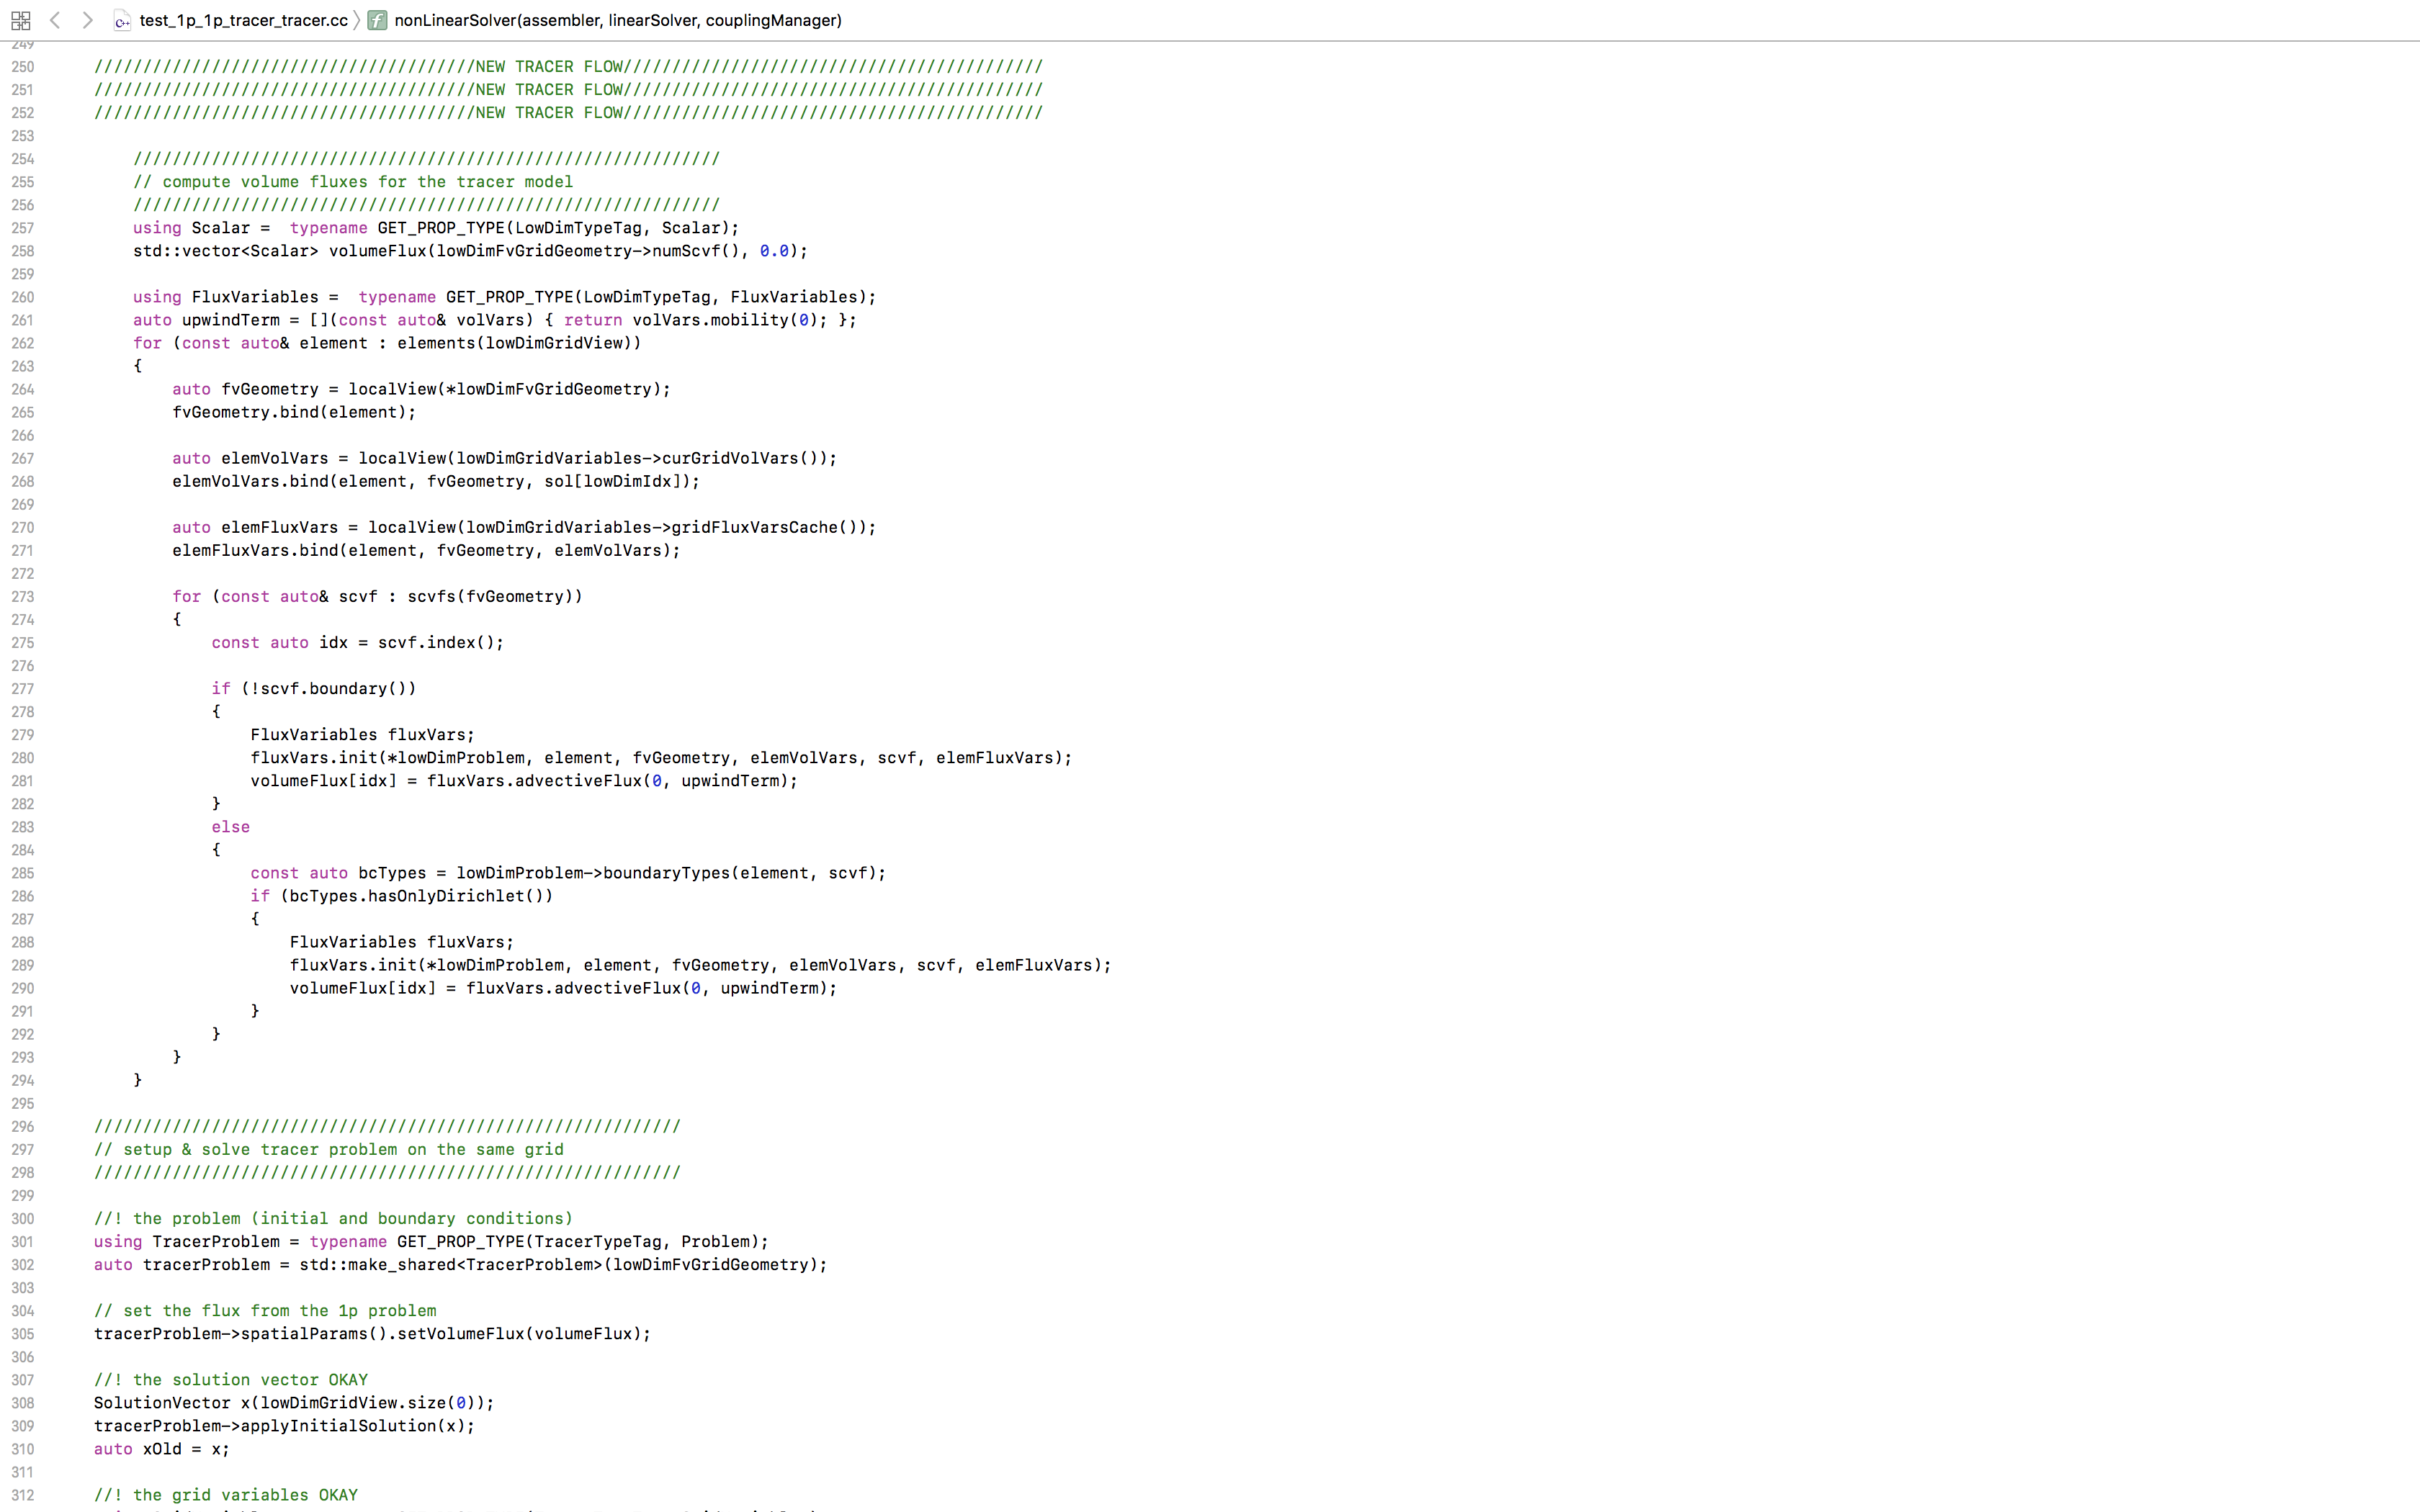
\includegraphics[width=350mm]{1p_1p_tracer_tracer_1}
\caption{\footnotesize The 1p-1p-tracer-tracer Code (1)}
\label{fig:1p-1p-tracer-tracer-1}
\end{figure}
\begin{figure}[h]
\centering
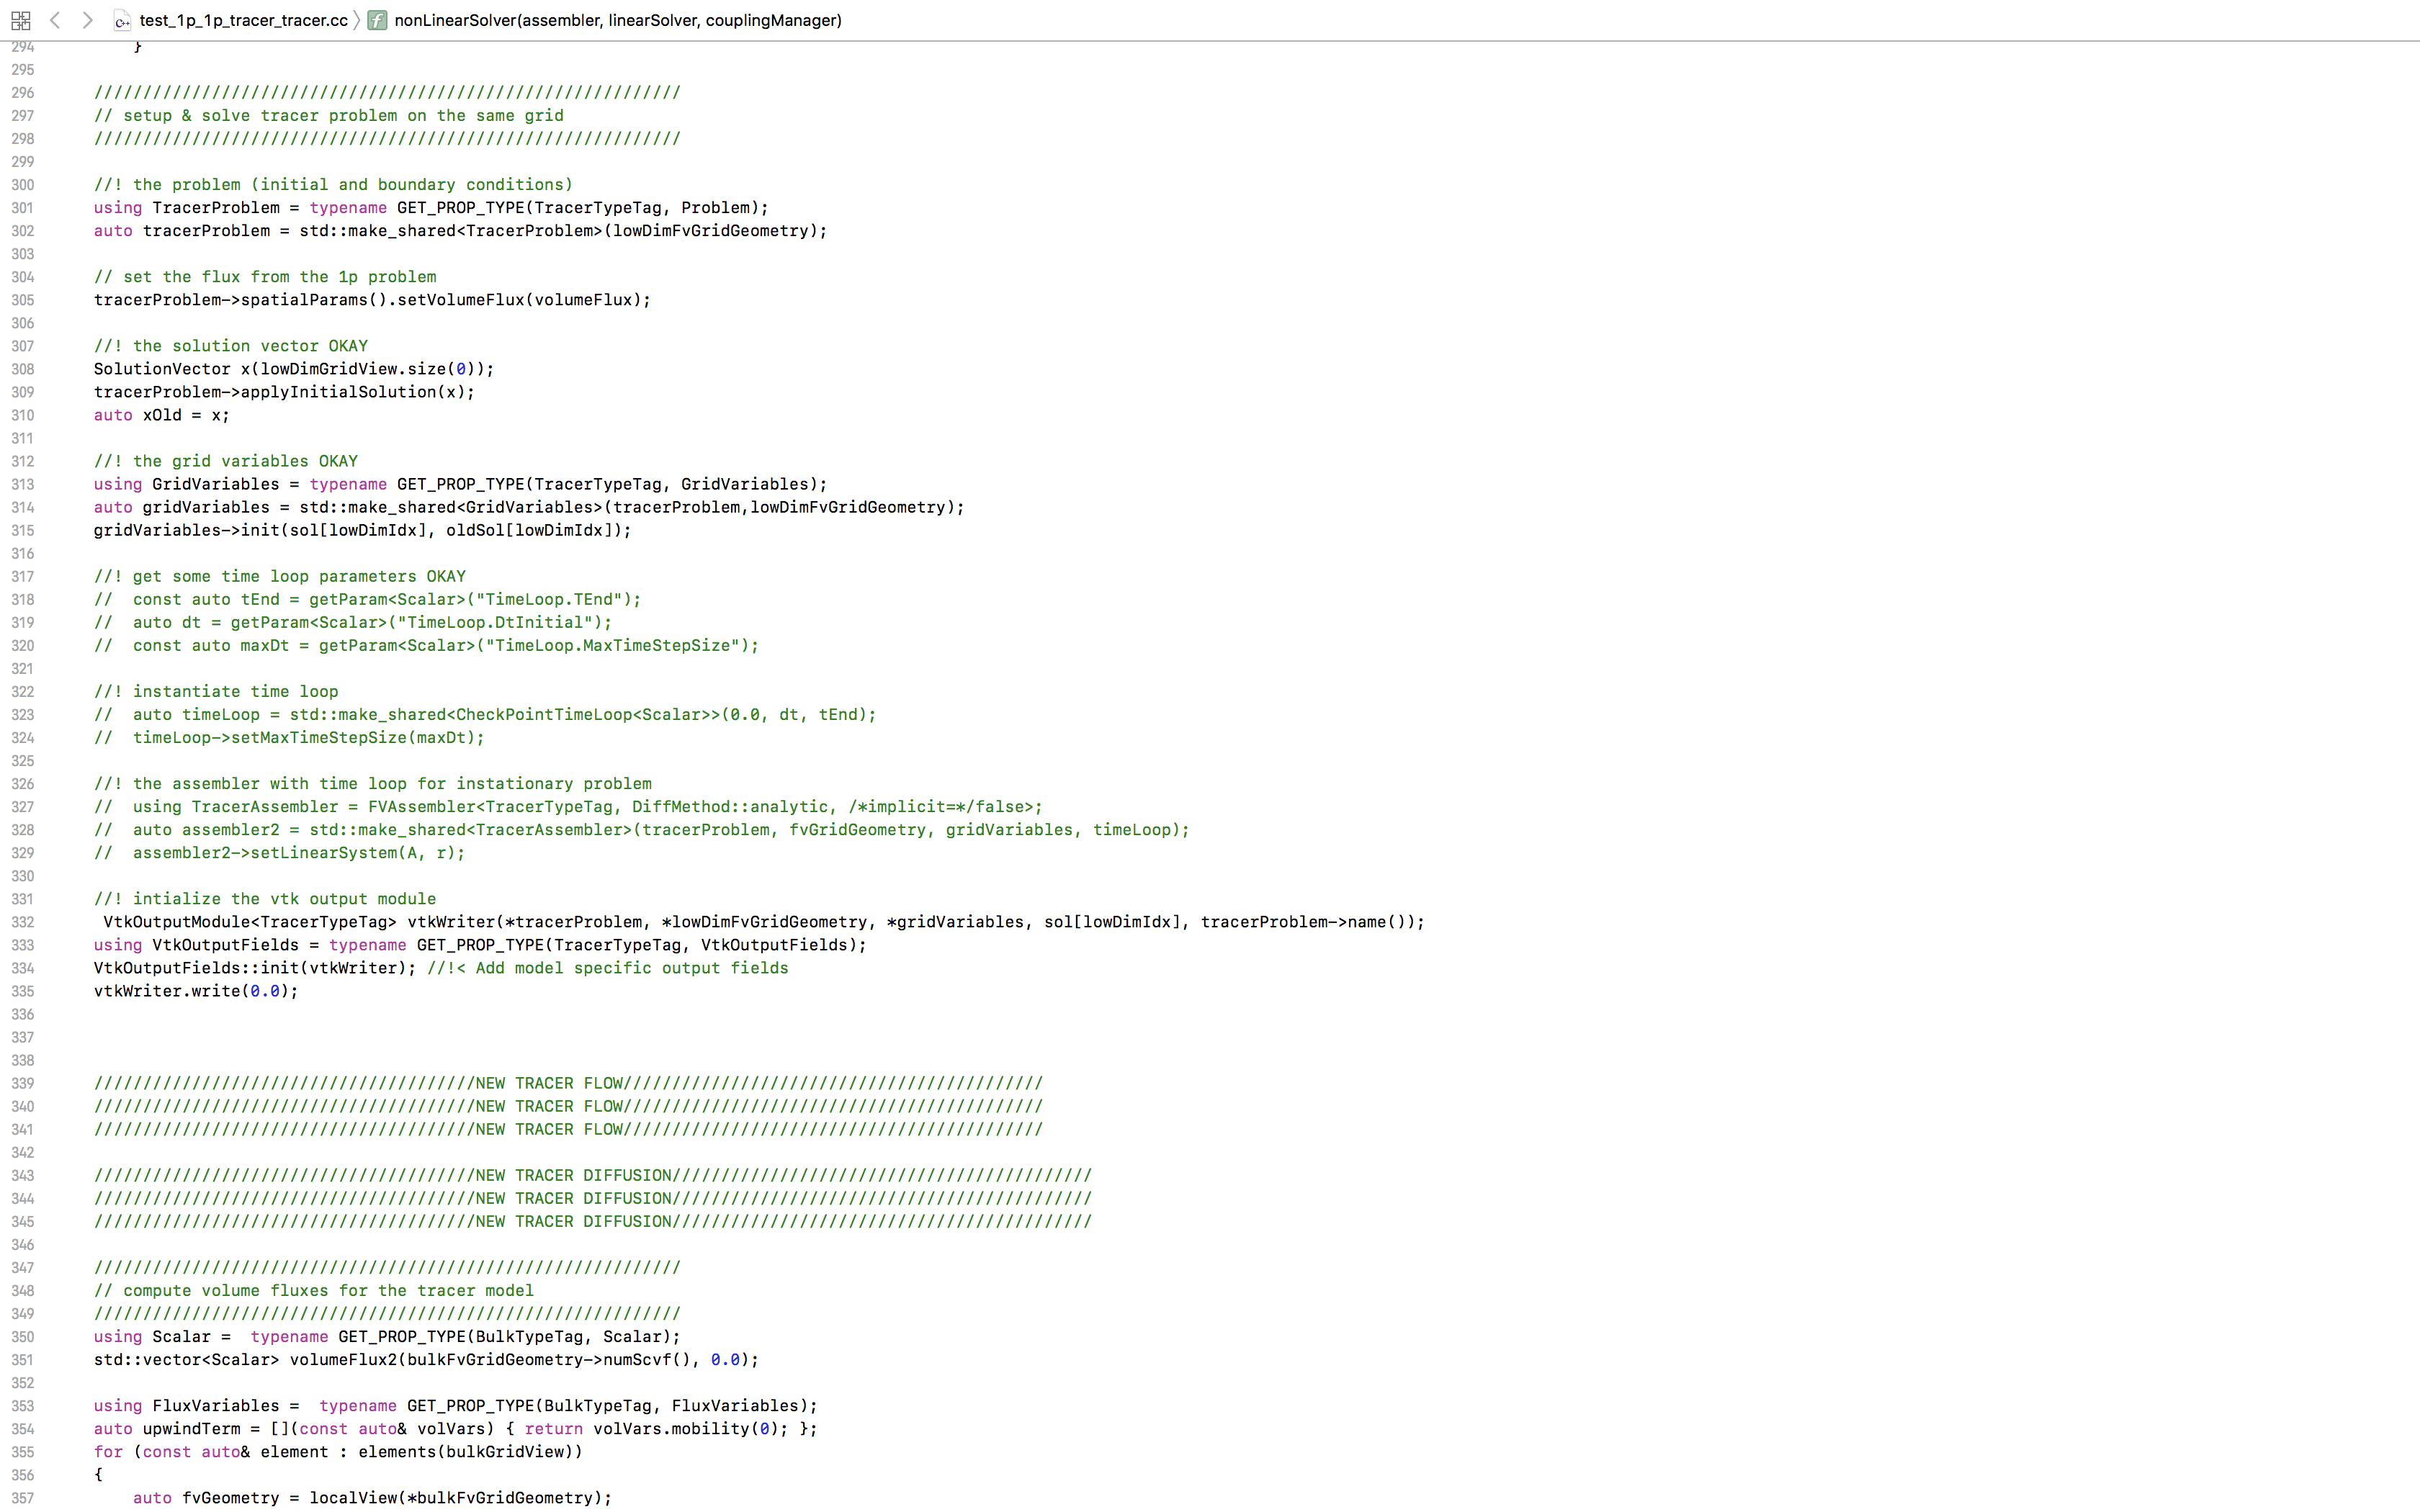
\includegraphics[width=350mm]{1p_1p_tracer_tracer_2}
\caption{\footnotesize The 1p-1p-tracer-tracer Code (2)}
\label{fig:1p-1p-tracer-tracer-2}
\end{figure}
%\begin{figure}[h]
%\centering
%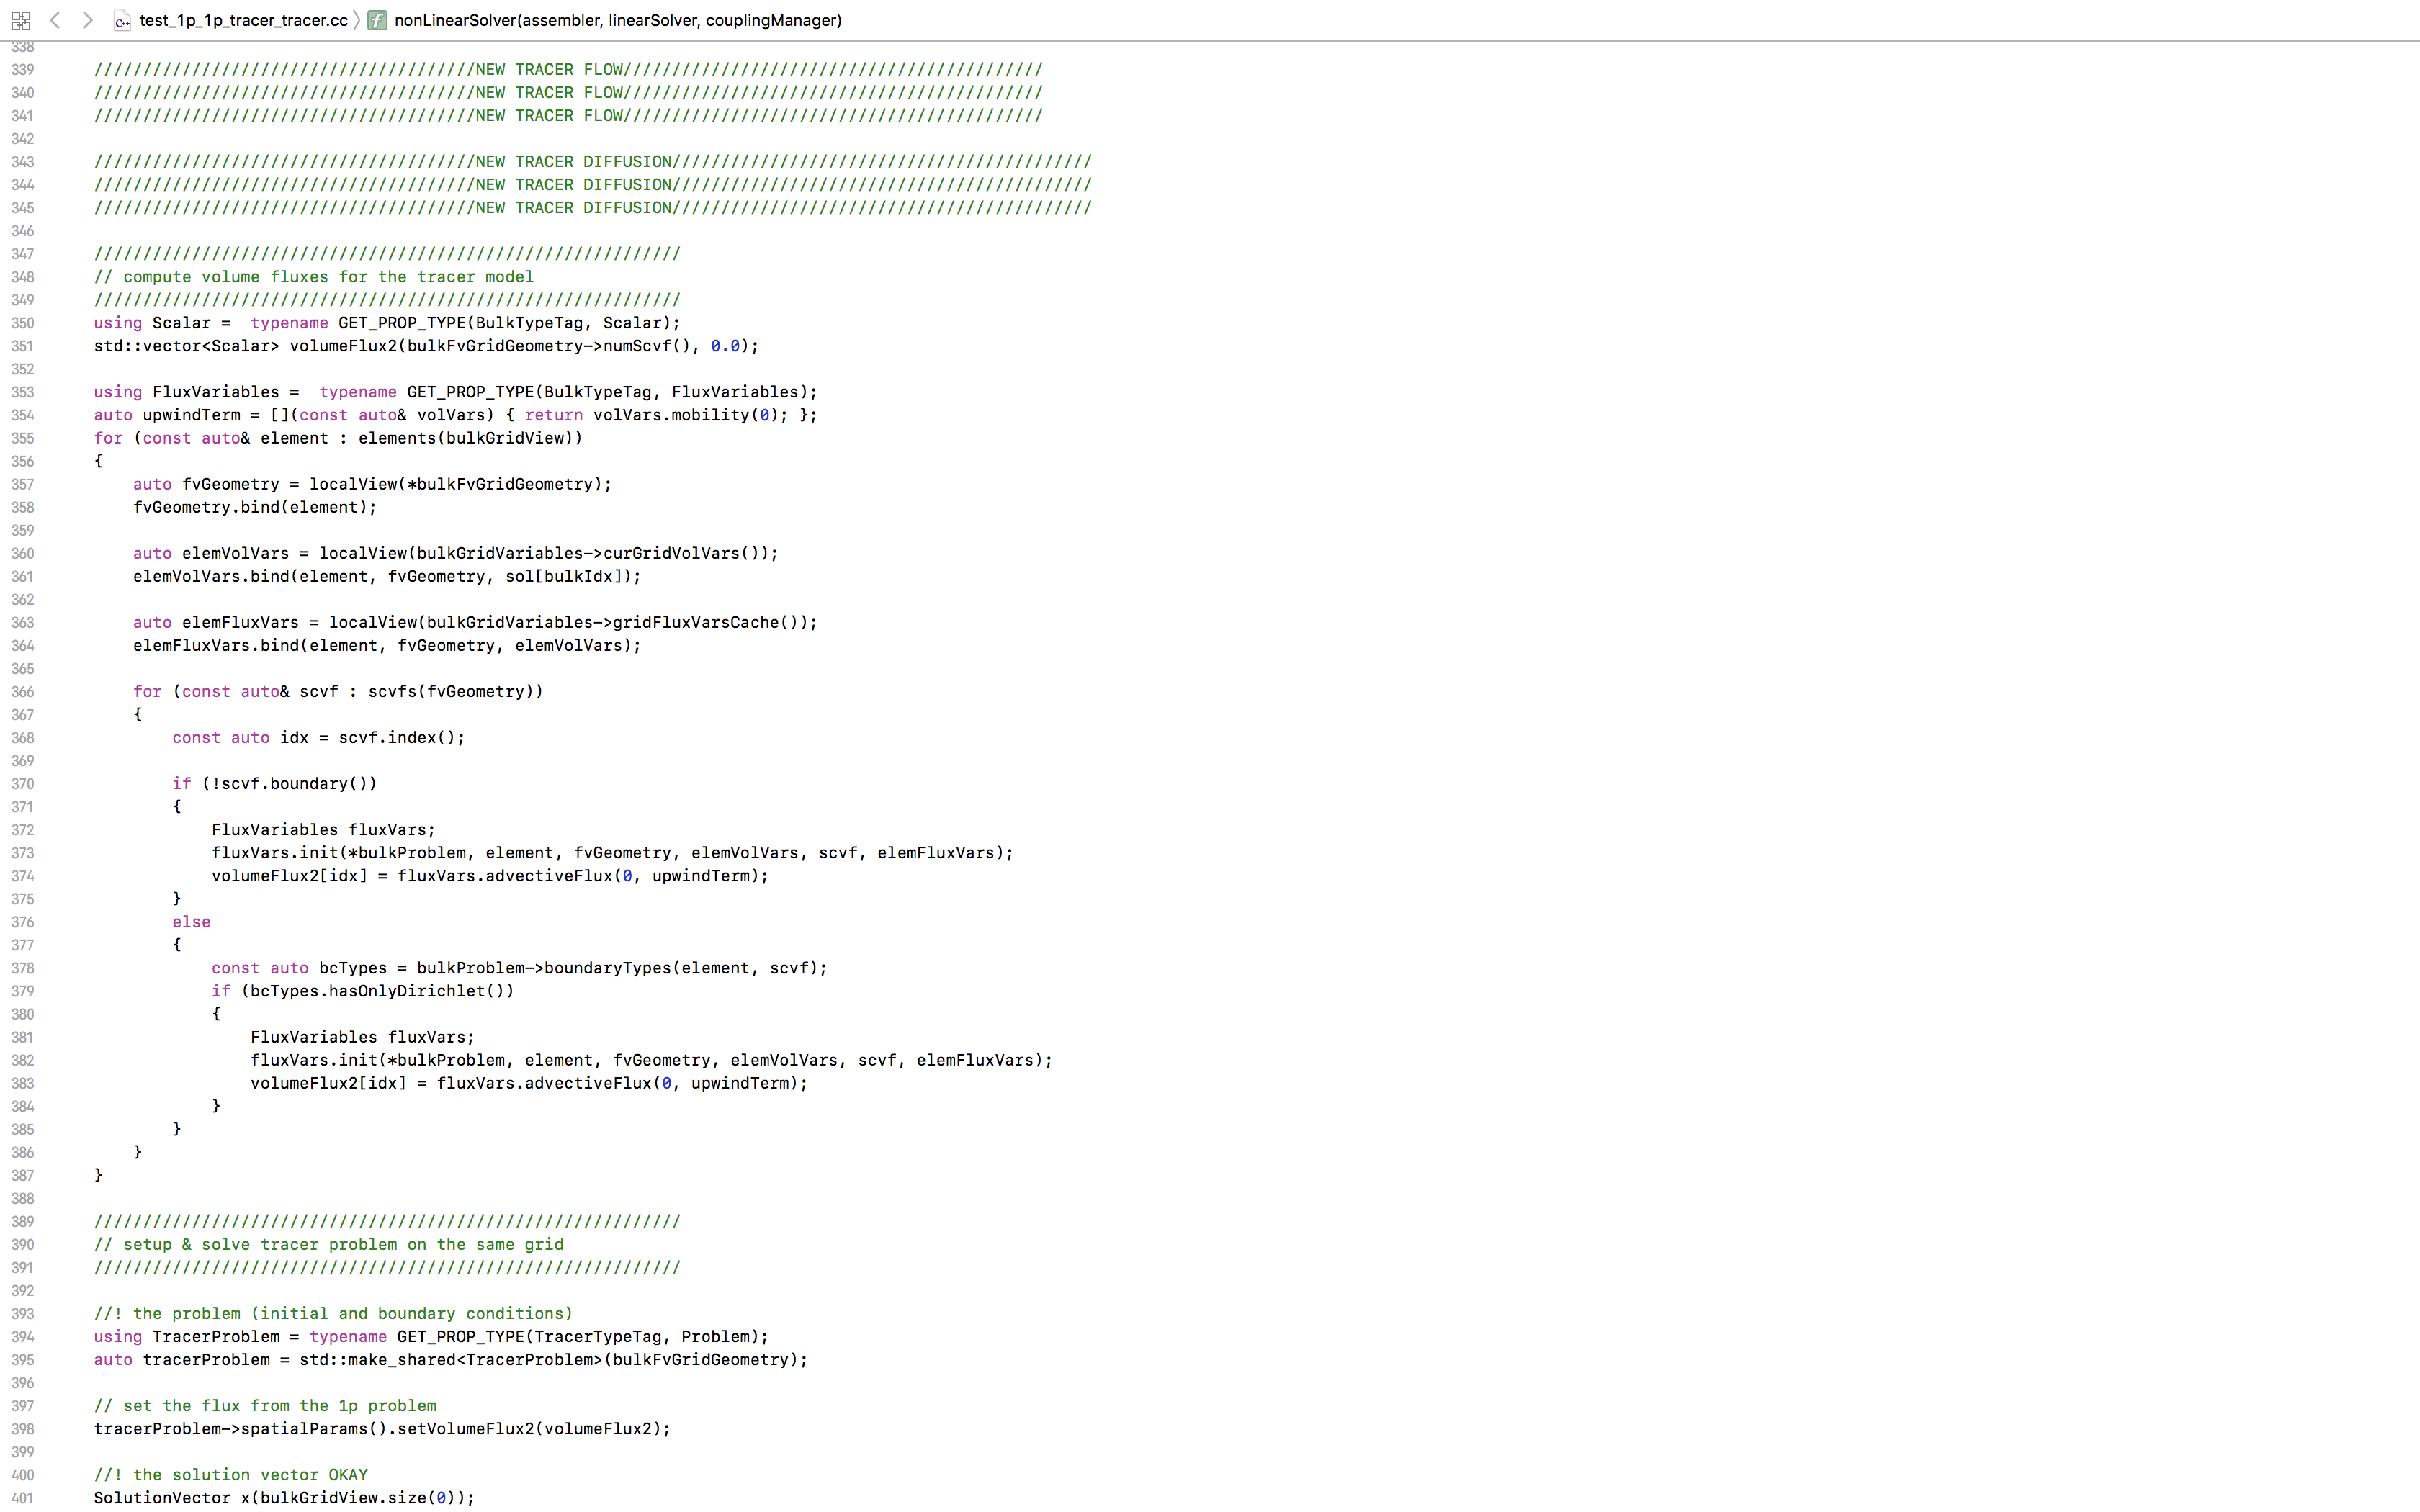
\includegraphics[width=350mm]{1p_1p_tracer_tracer_3}
%\caption{\footnotesize The 1p-1p-tracer-tracer Code (3)}
%\label{fig:1p-1p-tracer-tracer-3}
%\end{figure}
%\begin{figure}[h]
%\centering
%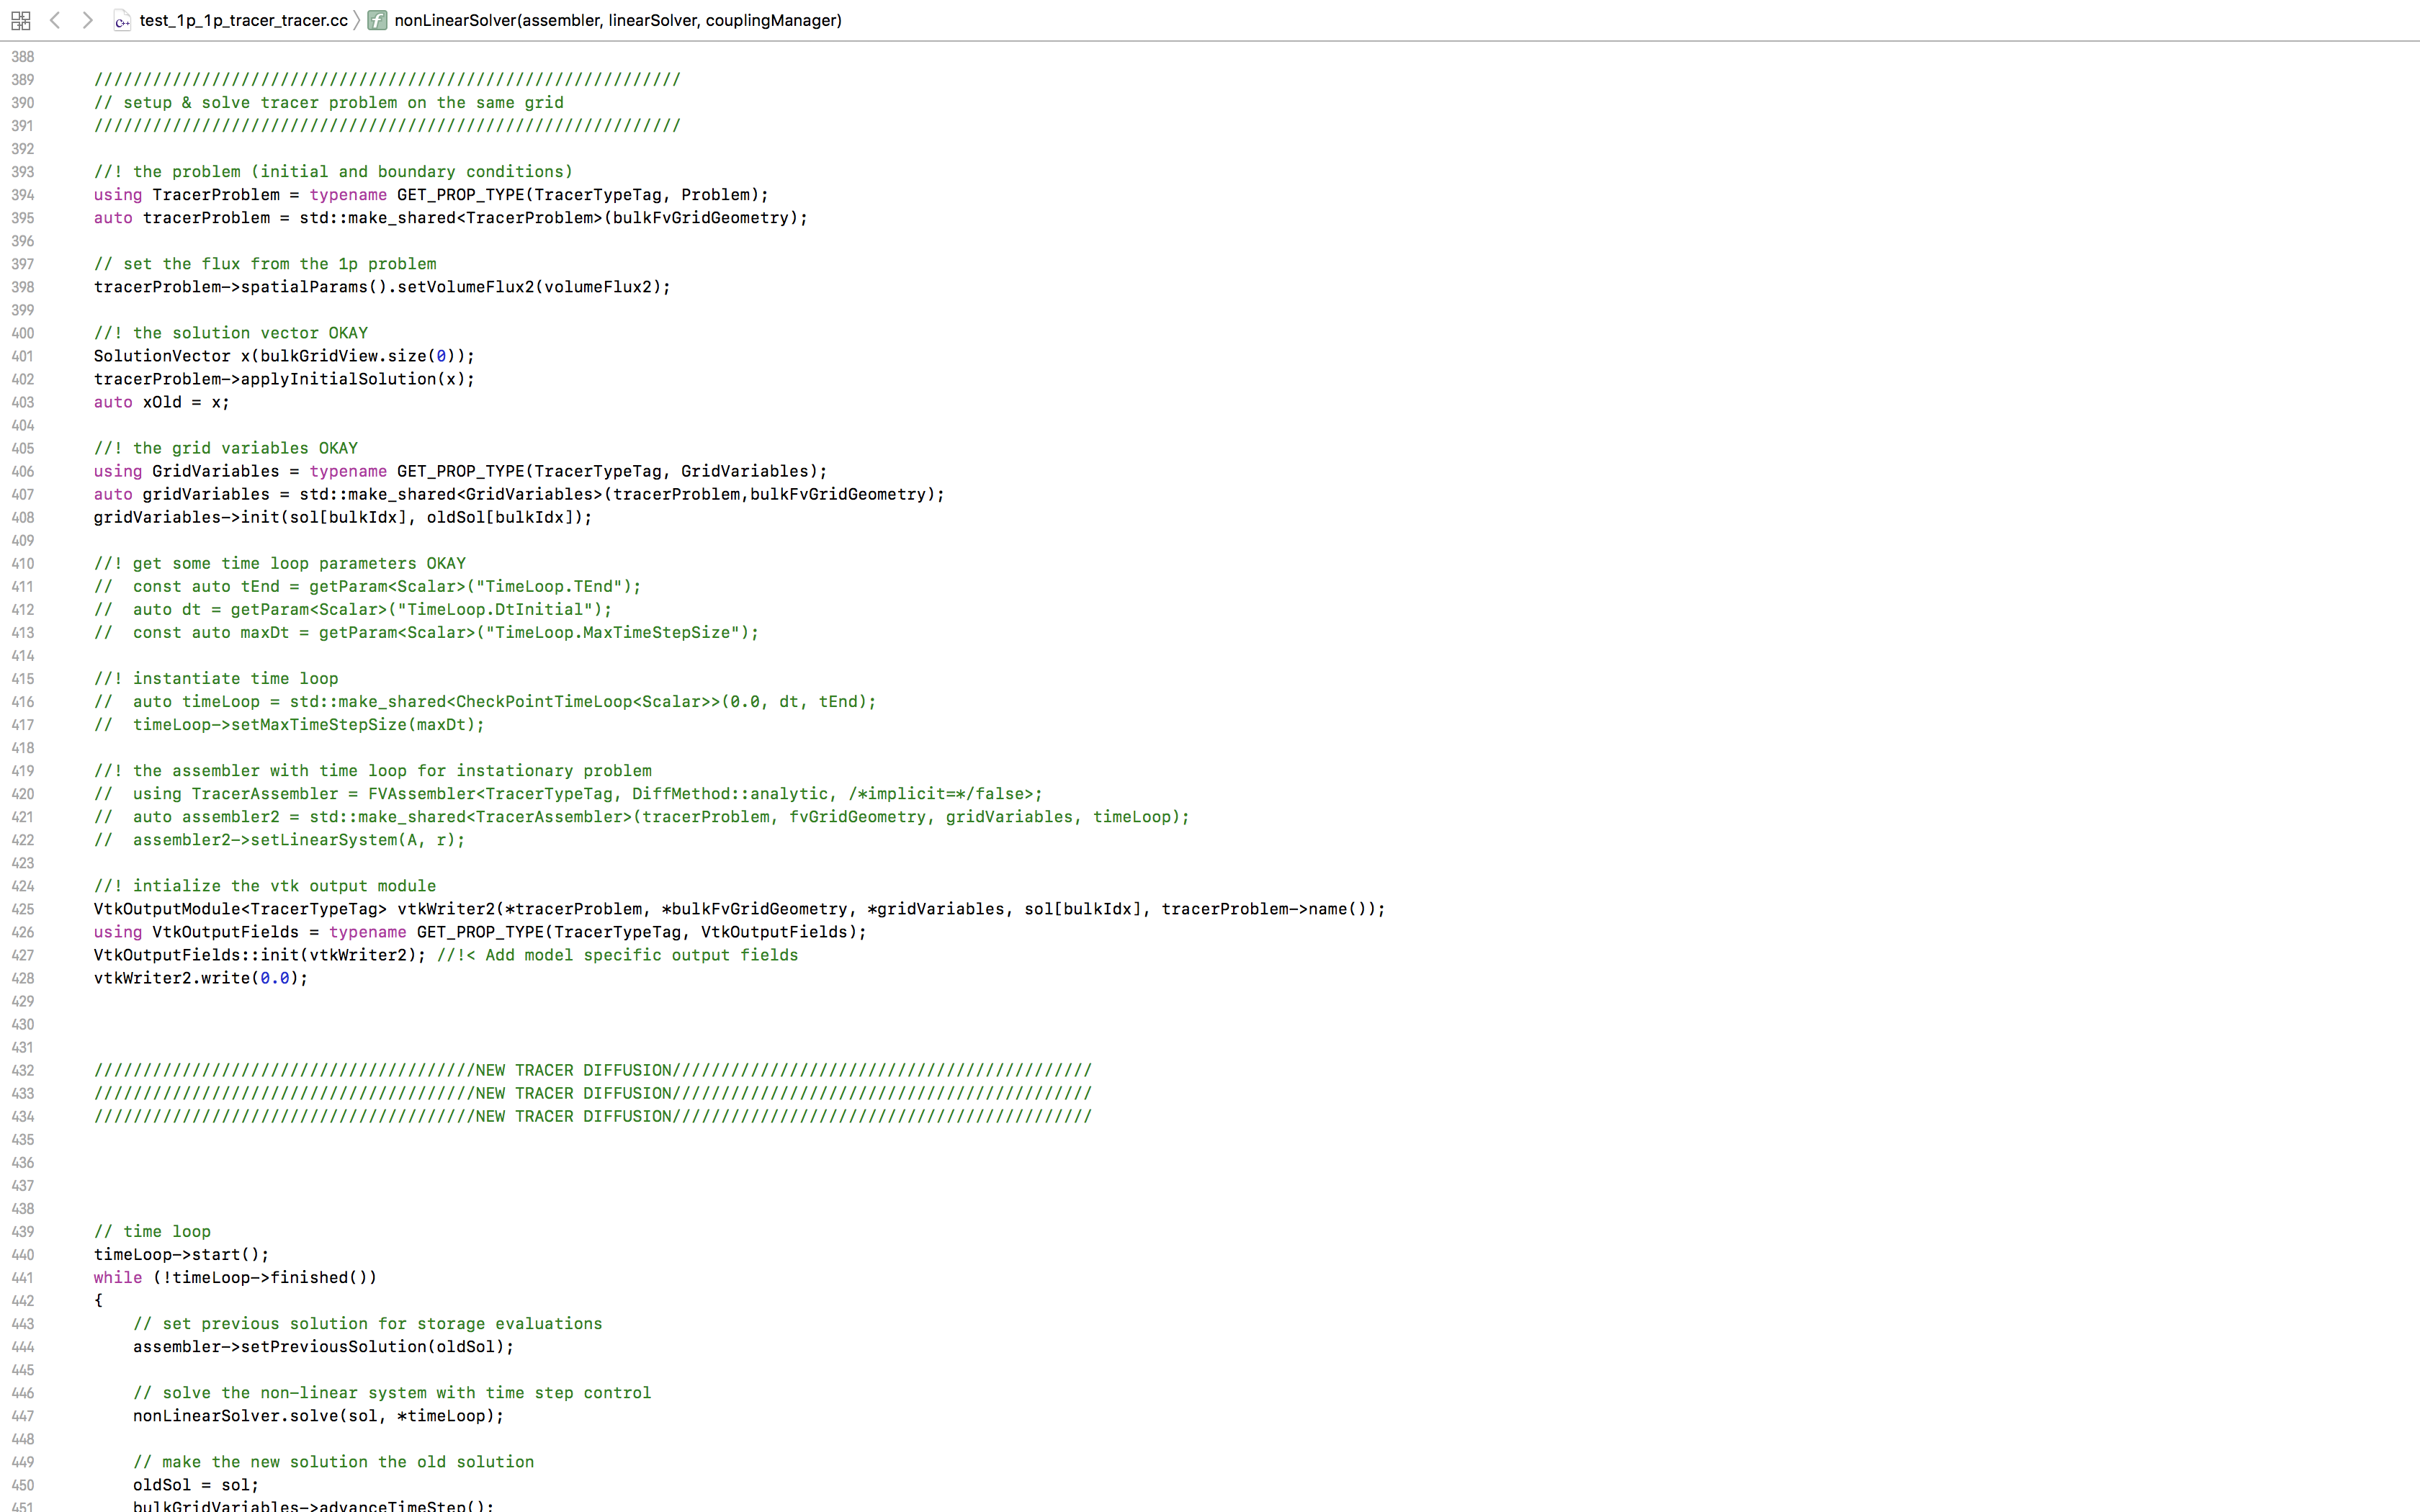
\includegraphics[width=350mm]{1p_1p_tracer_tracer_4}
%\caption{\footnotesize The 1p-1p-tracer-tracer Code (4)}
%\label{fig:1p-1p-tracer-tracer-4}
%\end{figure}

\subsubsection*{Some More Glomeruli}
\label{SomeMoreGlomeruli}

To picture the previously mentioned pressure computations on glomerular networks, the pressure field simulation result are shown from a second perspective. The figures \ref{fig:glom_pressure2}, \ref{fig:glom2_pressure2}, \ref{fig:glom3_pressure} and \ref{fig:glom4_pressure} show the simulation results for the Glomeruli 1, 2, 3 and 4.

%Glomerulus 1:
\begin{figure}[h]
\centering
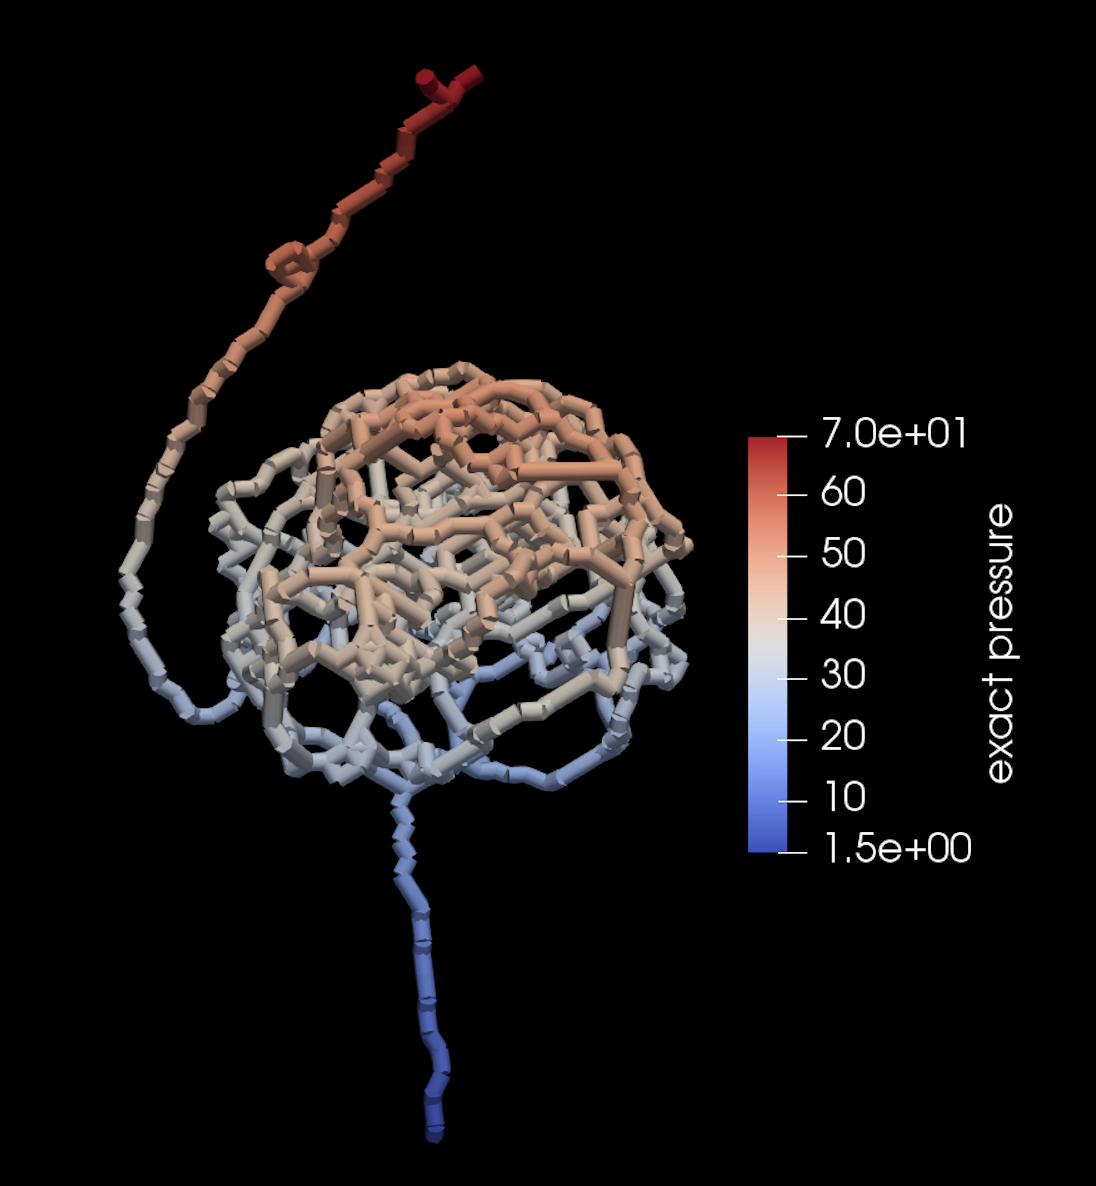
\includegraphics[width=162mm]{glom_pressure2}
\caption{Pressure Field in Glomerulus 1}
\label{fig:glom_pressure2}
\end{figure}
%Glomerulus 2:
\begin{figure}[h]
\centering
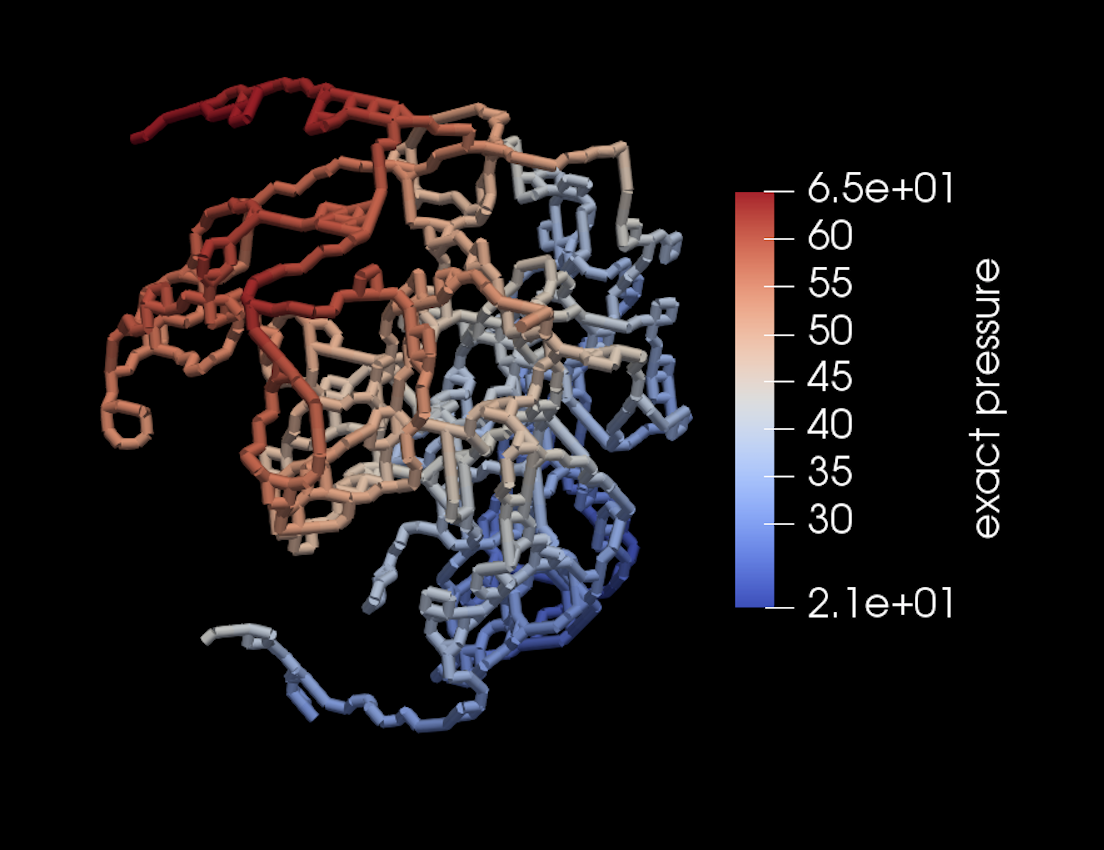
\includegraphics[width=162mm]{glom2_pressure2}
\caption{Pressure Field in Glomerulus 2}
\label{fig:glom2_pressure2}
\end{figure}
%Glomerulus 3:
\begin{figure}[h]
\centering
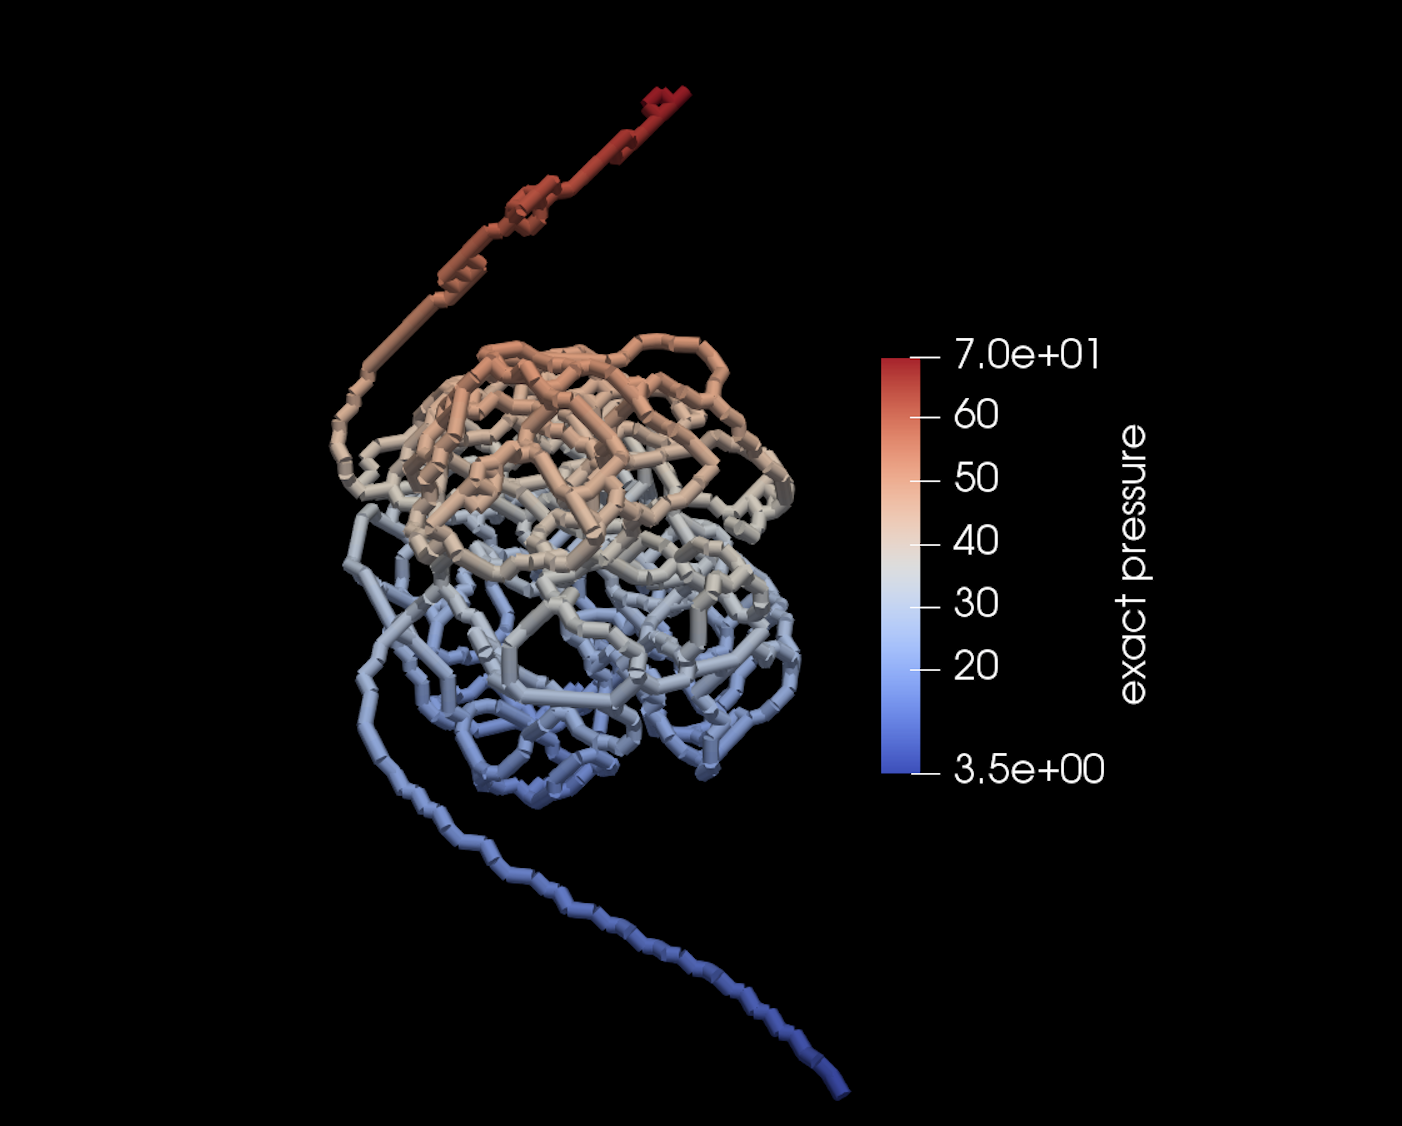
\includegraphics[width=162mm]{glom3_pressure}
\caption{Pressure Field in Glomerulus 3}
\label{fig:glom3_pressure}
\end{figure}
%Glomerulus 4:
\begin{figure}[h]
\centering
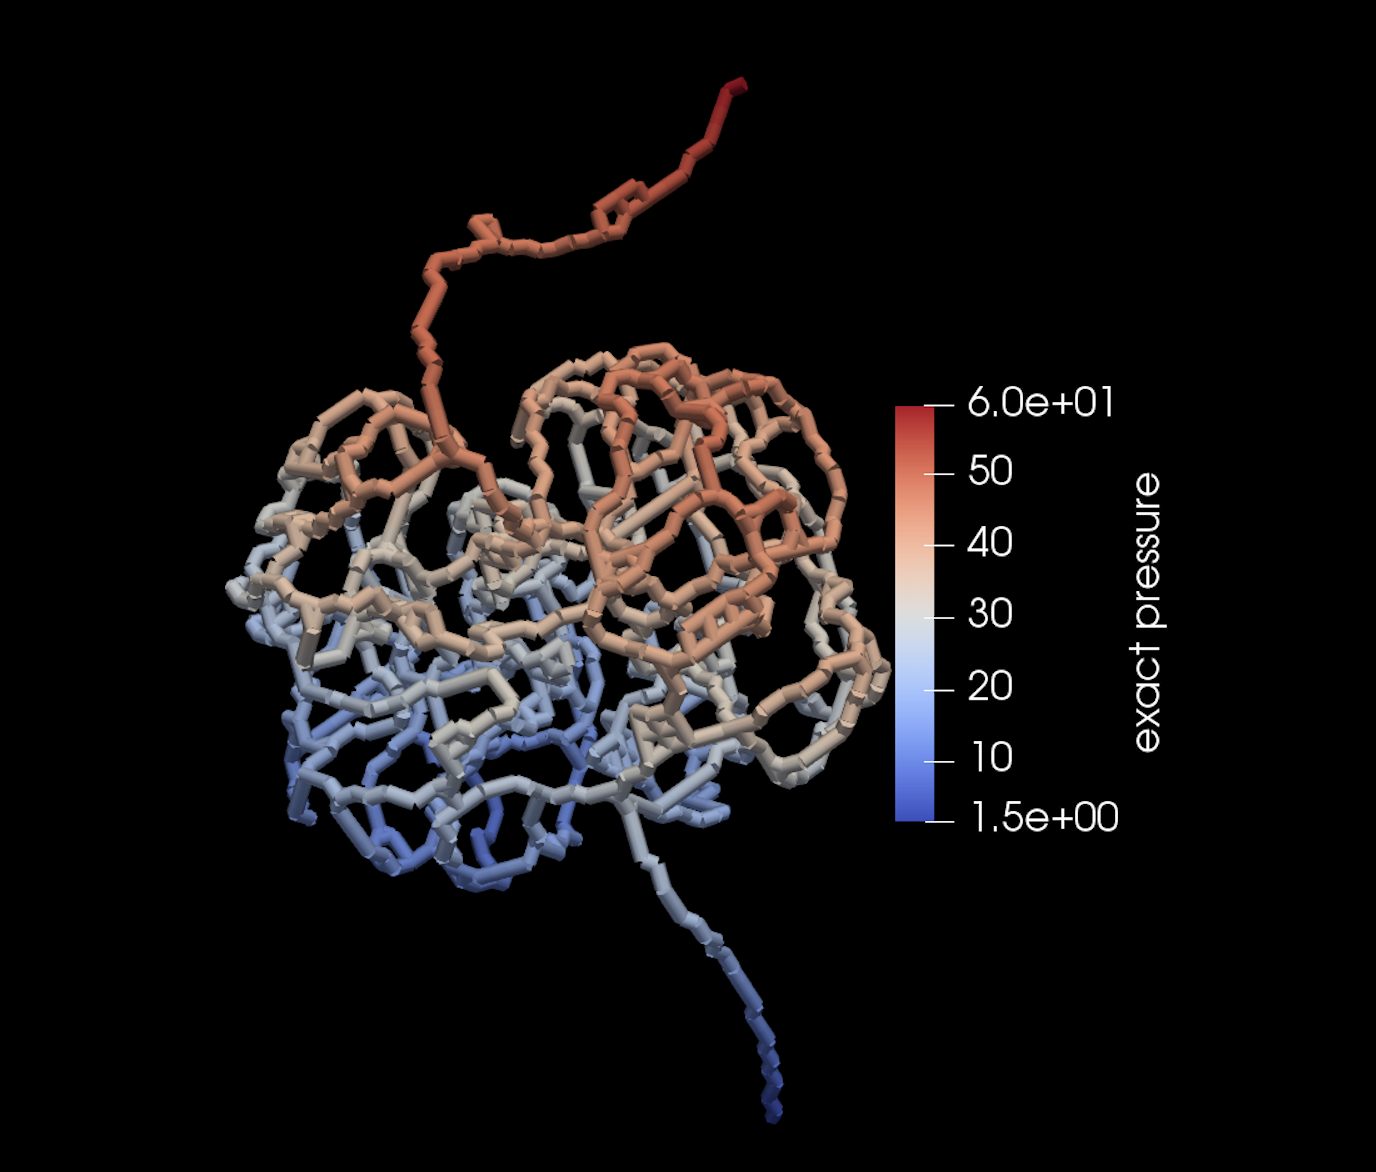
\includegraphics[width=162mm]{glom4_pressure}
\caption{Pressure Field in a Glomerulus 4}
\label{fig:glom4_pressure}
\end{figure}


\subsubsection*{Some Tracer Simulations}
\label{Tracer}

To give an example of what the tracer model is computing, a simulation of a simple diffusion of groundwater in a porous rock is given. The velocity field of the solute (Figure \ref{fig:tracer_velocity}) is assumed to be constant over the time. The solute field for the first time step can be seen on Figure \ref{fig:tracer_1}. The solute field in the rock for the last time step is visualized on Figure \ref{fig:tracer_2}.\\
Clearly the water has moved in the porous rock, and the solute field for the last time step is different than the field in the first time step. The solute is \emph{traced} in the given domain, and a solute field for each time step is computed.\\
I attached these images to qualitatively give the reader an insight into how the tracer works, and what the idea behind tracing oxygen in the tissue, in order obtain oxygen fields, was.
\begin{figure}[h]
\centering
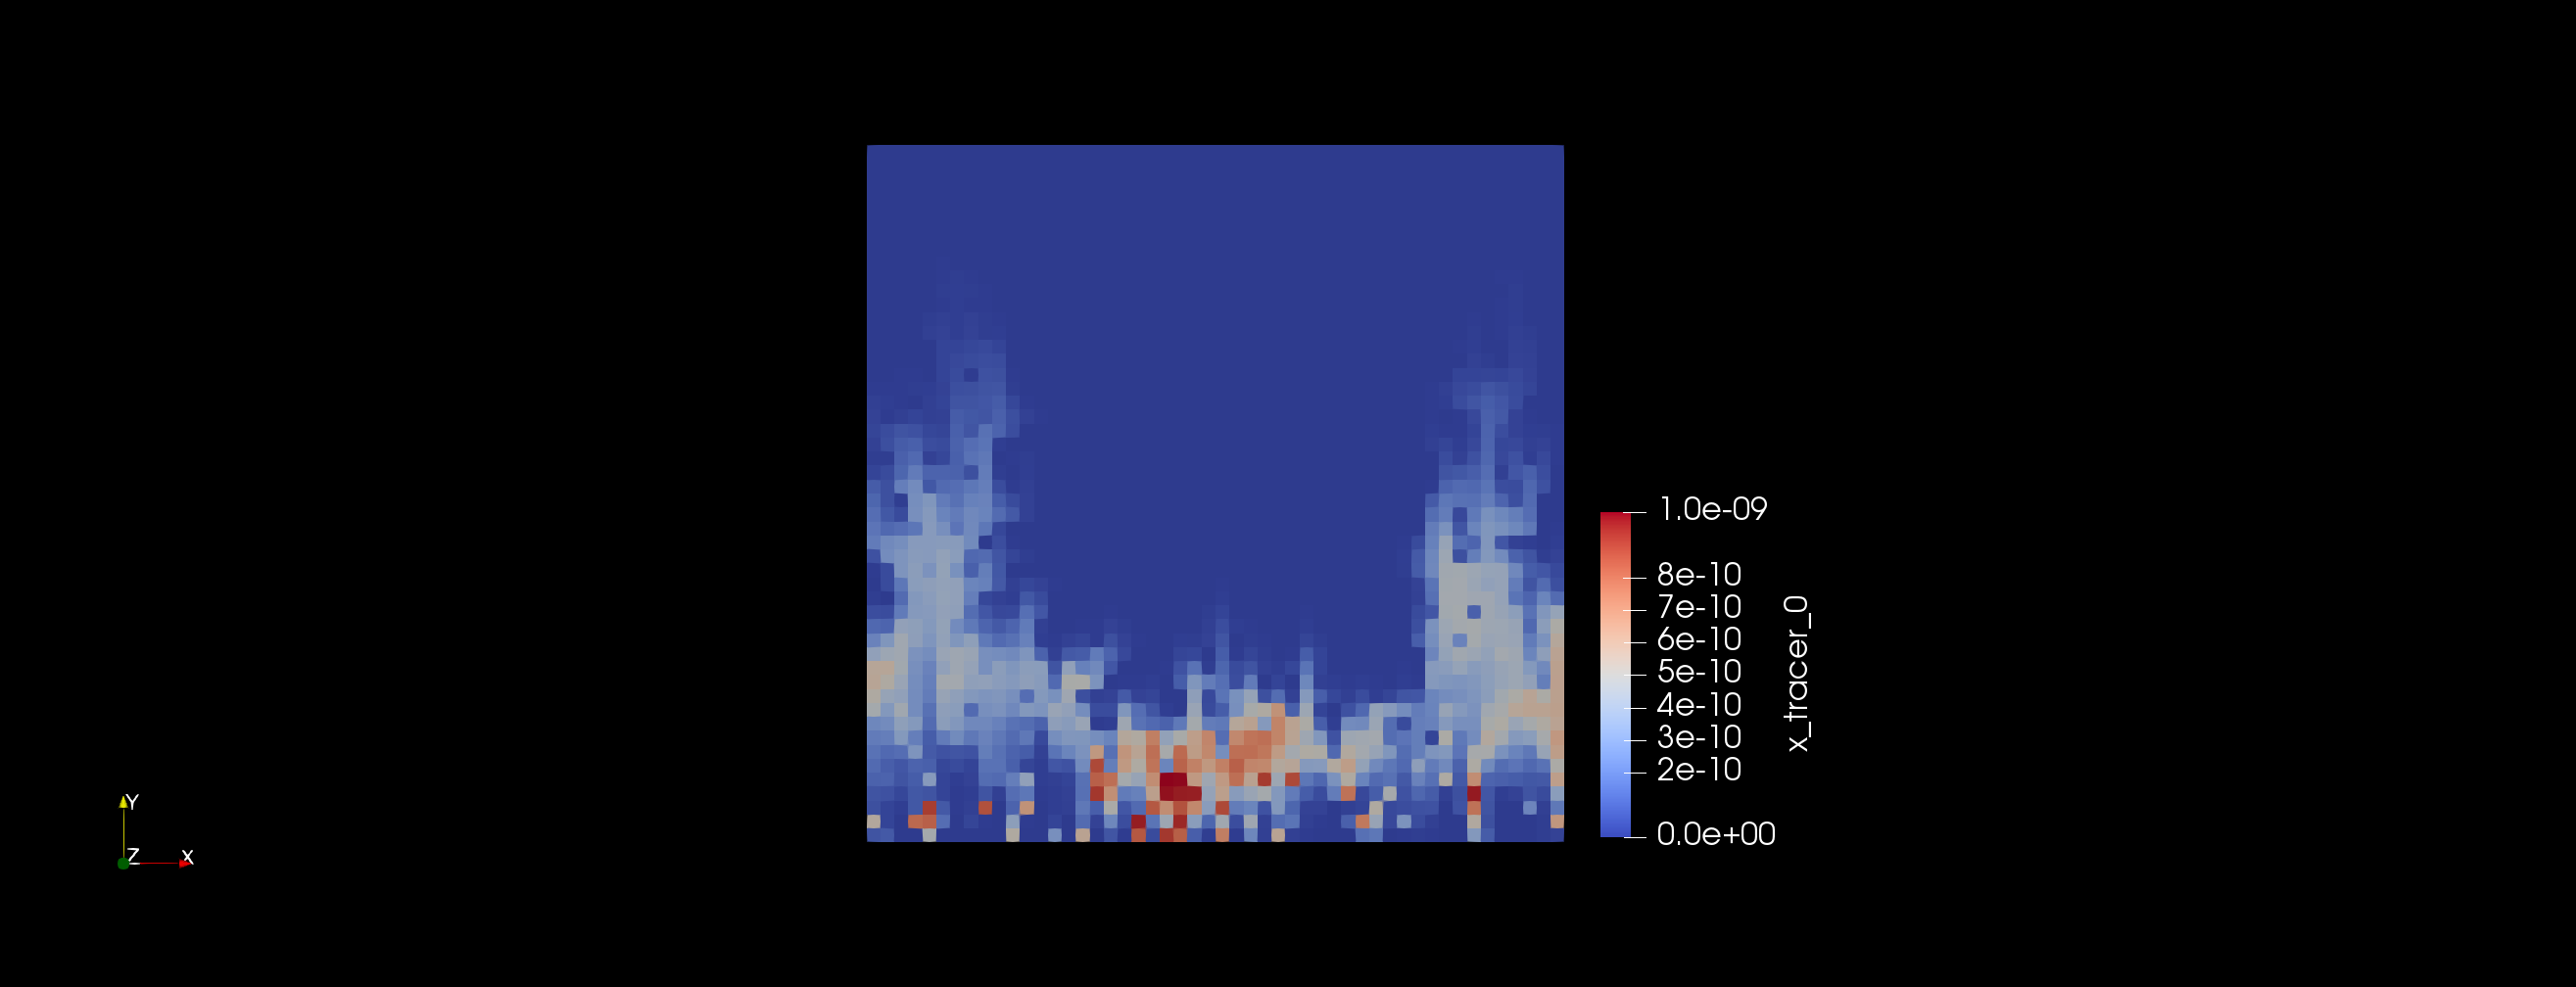
\includegraphics[width=162mm]{tracer_1}
\caption{\footnotesize $DuMu^x$ Tracer Concentration Simulation for a Rectangular Geometry (Time Step 1)}
\label{fig:tracer_1}
\end{figure}
\begin{figure}[h]
\centering
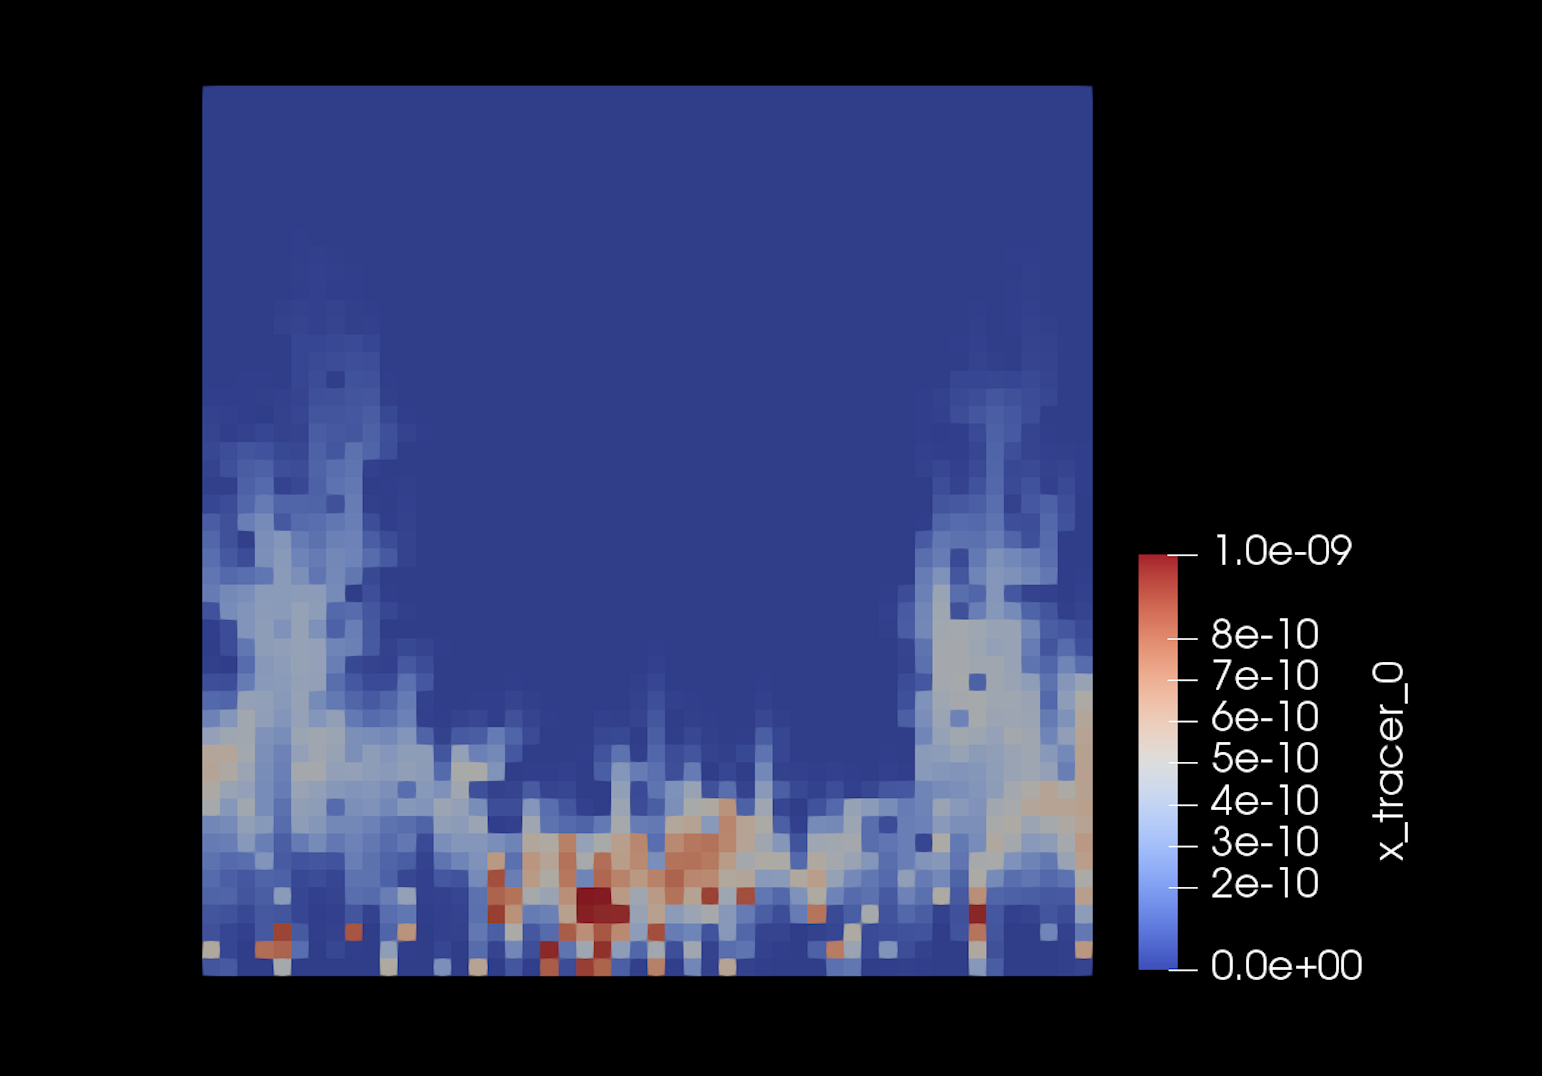
\includegraphics[width=162mm]{tracer_2}
\caption{\footnotesize $DuMu^x$ Tracer Concentration Simulation for a Rectangular Geometry (Time Step 10)}
\label{fig:tracer_2}
\end{figure}
\begin{figure}[h]
\centering
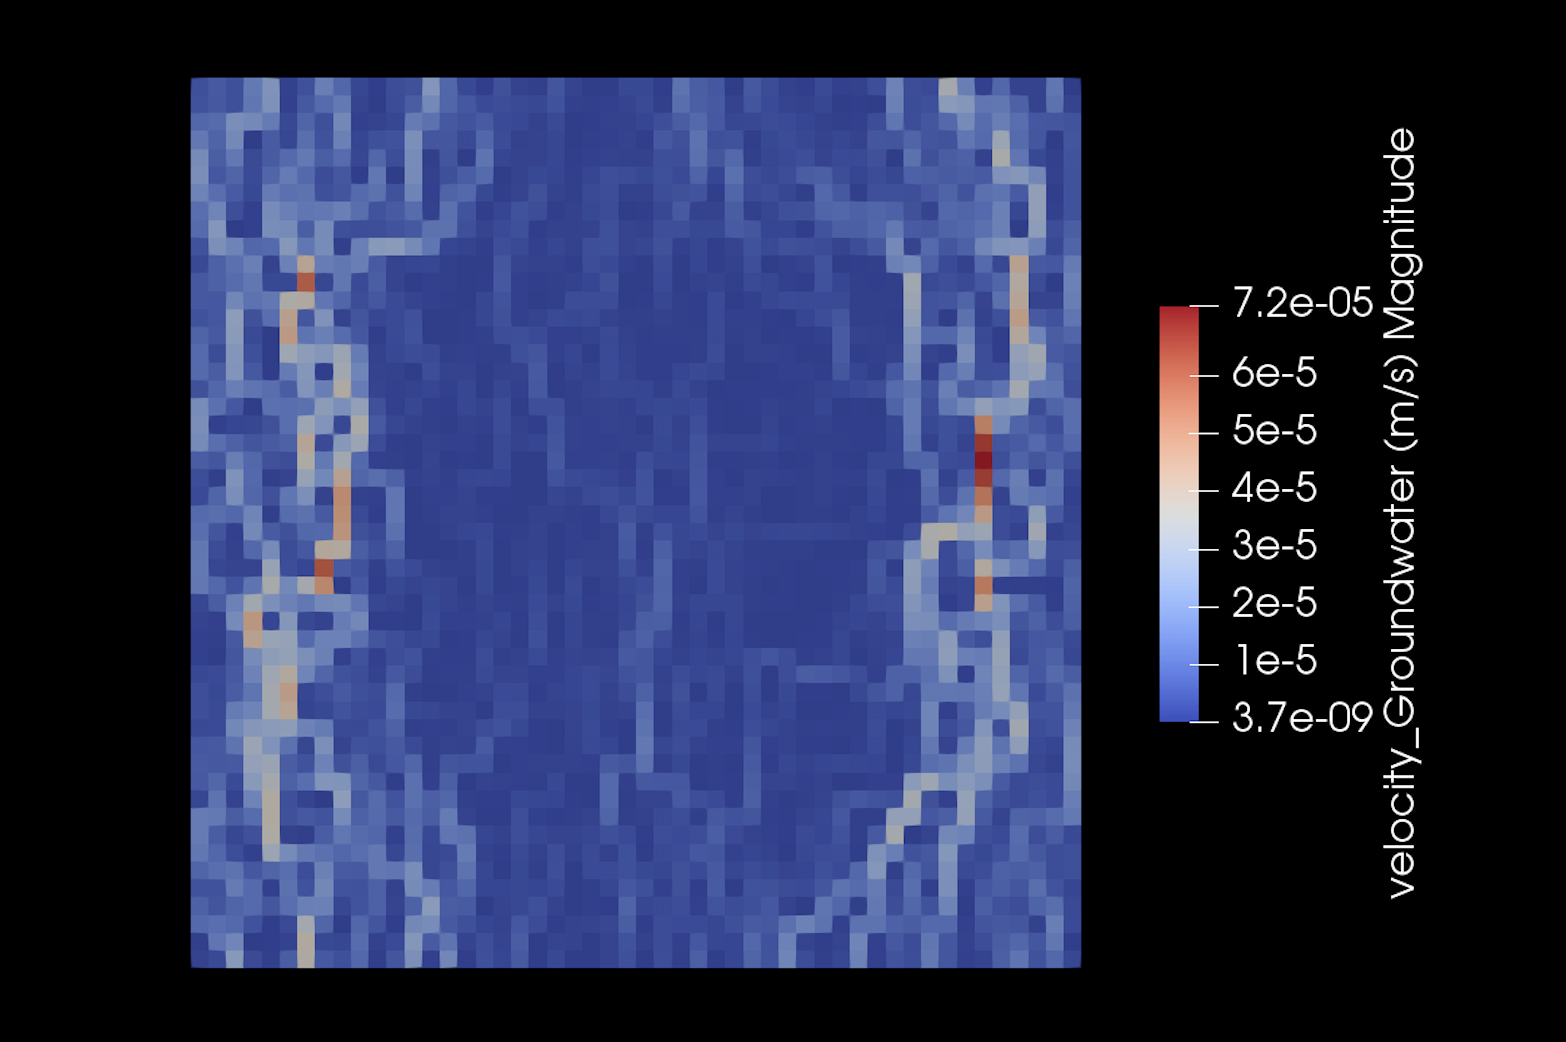
\includegraphics[width=162mm]{tracer_velocity}
\caption{\footnotesize $DuMu^x$ Tracer Velocity Simulation for a Rectangular Geometry}
\label{fig:tracer_velocity}
\end{figure}